\section{FITTING METHODOLOGIES AND STABILITY ANALYSIS}
\label{sec:fitting_methodologies}

The lattice data show different levels of statistical precision among the invariant amplitudes. The real part of the unpolarized amplitude, $\tAmp_{2B}^{\text{Re}}$, has small statistical uncertainties across the simulated position space, whereas the imaginary unpolarized amplitude $\tAmp_{2B}^{\text{Im}}$ and the real Sivers amplitude $\tAmp_{12B}^{\text{Re}}$ have larger gauge noise. We already discarded the imaginary Sivers amplitude $\tAmp_{12B}^{\text{Im}}$ because it is consistent with zero. We first establish a stable global fit for $\tAmp_{2B}^{\text{Re}}$ as the baseline for the remaining numerical analysis, as it corresponds to the leading-twist unpolarized TMD and has the highest data quality.

We parameterize the amplitudes natively in the Cartesian space $(b_L, b_T)$ rather than the Lorentz-invariant variable space $(P \cdot b, b^2)$. Fitting in $(b_L, b_T)$ provides a larger, more uniformly distributed set of discrete data points and resolves kinematic degeneracies. Because the squared separation distance $b^2 = b_L^2 + b_T^2$ is strictly non-negative, multiple distinct combinations of longitudinal and transverse separations (such as a large $b_L$ with a small $b_T$, or a small $b_L$ with a large $b_T$) map to the same invariant $b^2$. So, fitting in the $(P \cdot b, b^2)$ basis would compress these distinct orthogonal spatial dependencies into a single coordinate. Fitting over the $(b_L, b_T)$ grid allows the model to separate the longitudinal decay profile from the transverse decay profile. 

The fitting and stability analysis in this chapter follows a sequential progression towards finding the final model. In Section~\ref {sec:gaussian_transformation}, we demonstrate why the simple Gaussian ansatz fails due to non-integrable longitudinal growth ($\alpha < \beta$). In Section~\ref{sec:discretization_effects}, we isolate ultraviolet lattice discretization artifacts by applying a spatial cutoff $|\vect{b}| \ge 3a$. In Section~\ref{sec:pysr_methodology}, using genetic programming with an asymptotic decay penalty, we discover the generalized Lorentzian power-law tail $(1+b^2)^{-j}$ and the exponential area-law factor $e^{-f\eta}$. In Sections~\ref{sec:rejection_exponential_longitudinal} and~\ref{sec:factorized_ansatze_failure}, We test factorized models across all three surviving amplitudes, showing that while they describe $\tAmp_{2B}^{\text{Re}}$, they fail on $\tAmp_{2B}^{\text{Im}}$ and $\tAmp_{12B}^{\text{Re}}$, requiring the coupled denominator $[1 + c(P\cdot b)^2/P_L^2 + d b^2]^j$. Then in Sections~\ref{sec:asymptotic_eta_anti_quark} and~\ref{sec:candidate_selection}, we analyze parameter behavior across individual staple extents $\eta \in [6, 10]$, select the asymptotic model $c(\eta) = c(1 - k_1/\eta - k_2/\eta^2)$ based on AIC, and enforce physical anti-quark suppression at large negative $x$ ($x < -0.2$). Finally, in Section~\ref{sec:simultaneous_fit_strategy}, we perform a correlated Jackknife $\chi^2$ minimization across all amplitudes, cancel the shared $e^{-f\eta}$ factor, and extract the $x$-dependent Sivers shift.

\subsection{Failure of Simple Gaussian Model}
\label{sec:gaussian_transformation}

For the real parts of the amplitudes ($\tAmp^{Re}_{iB}$), Hermitian conjugation symmetries require the function to be even in the longitudinal separation $b_L$. We model the real amplitude with a standard 2D Gaussian centered at the origin
\begin{align}
    \tAmp^{Re}_{iB}&=\gamma \exp{\left[-\alpha b_L^2-\beta b_T^2\right]}
\end{align}
To transform this into the invariant variable space, we use the lattice four-vector square, $b^2 = b_L^2 + b_T^2$, to substitute $b_T^2 = b^2 - b_L^2$ and also apply the Lorentz-invariant projection derived in Section \ref{sec:lorentz_mapping}, where the longitudinal spatial coordinate is given by $b_L = (P \cdot b) / (-P_L)$. Squaring this substitution gives
\begin{align}
   \tAmp^{Re}_{iB} &=\gamma \exp{\left[-\frac{\left(\alpha-\beta\right)}{P_{L}^2} (P\cdot b)^{2}-\beta b^{2}\right]}
\end{align}

For the Fourier integral $\int d(P\cdot b) e^{ix(P\cdot b)} \tAmp_{iB}$ to converge, the argument of the exponential must remain negative as $(P \cdot b) \to \pm \infty$. This requires $(\alpha - \beta) > 0$. If $\alpha < \beta$, the amplitude grows exponentially at large longitudinal separations, making the integral divergent.

Fitting this Gaussian model to our lattice data yields $\alpha < \beta$ for the unpolarized real amplitude, $\tAmp^{Re}_{2B}$. 
\begin{figure}[H]
    \centering
    % Left Column: Re A2B
    \begin{minipage}{0.48\textwidth}
        \centering
        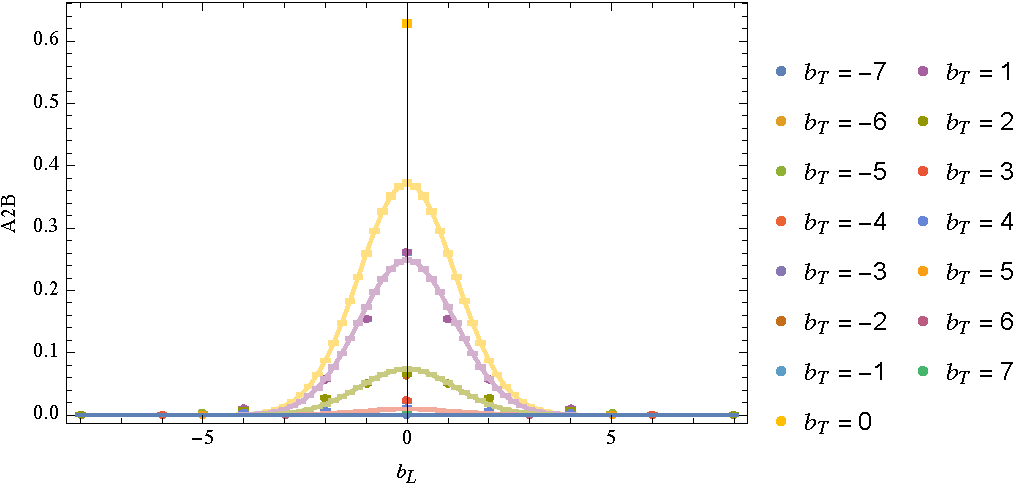
\includegraphics[width=\linewidth]{plots/Gaussian_fit_all_b/Gaussian_A2B_Re_P1_FailedFit.pdf}\\[2ex]
        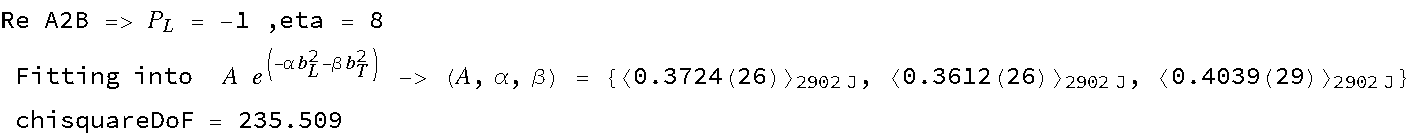
\includegraphics[width=\linewidth]{plots/Gaussian_fit_all_b/Gaussian_A2B_Re_P1_FailedFit_details1.pdf}\\[2ex]
        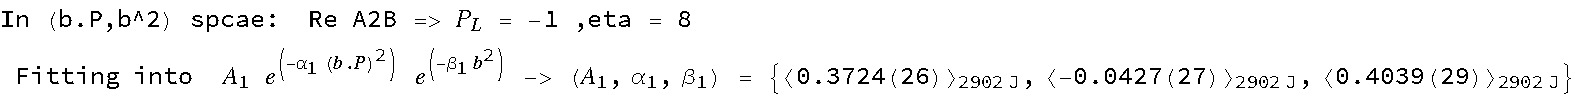
\includegraphics[width=\linewidth]{plots/Gaussian_fit_all_b/Gaussian_A2B_Re_P1_FailedFit_details2.pdf}
    \end{minipage}\hfill
    % Right Column: Re A12B
    \begin{minipage}{0.48\textwidth}
        \centering
        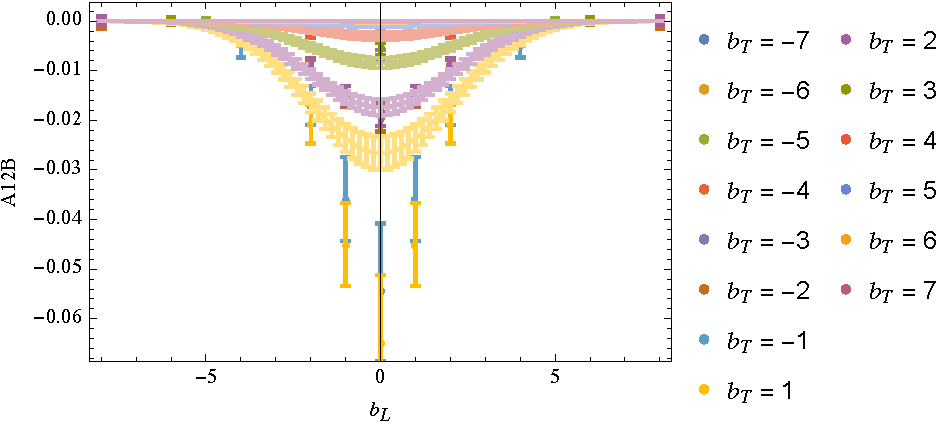
\includegraphics[width=\linewidth]{plots/Gaussian_fit_all_b/Gaussian_A12B_Re_P1_FailedFit.pdf}\\[2ex]
        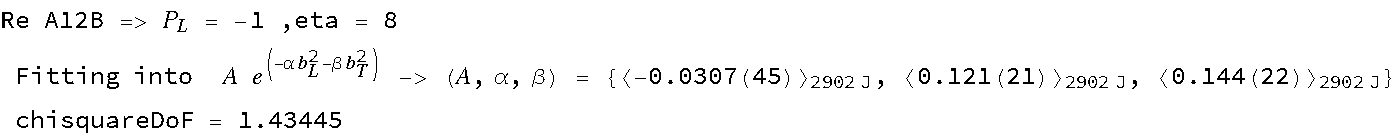
\includegraphics[width=\linewidth]{plots/Gaussian_fit_all_b/Gaussian_A12B_Re_P1_FailedFit_details1.pdf}\\[2ex]
        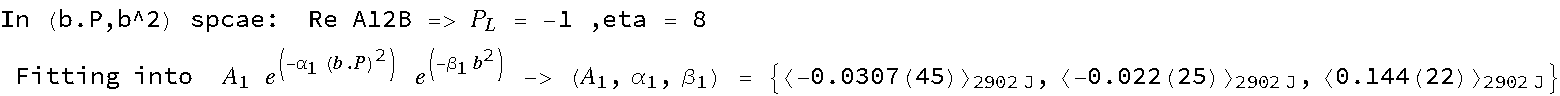
\includegraphics[width=\linewidth]{plots/Gaussian_fit_all_b/Gaussian_A12B_Re_P1_FailedFit_details2.pdf}
    \end{minipage}
    \caption{Failure of Gaussian model fit for $\tAmp^{Re}_{2B}$ (with $\alpha-\beta = -0.0427(27)$ and $\chi^2/\text{dof}\approx 235$) and $\tAmp^{Re}_{12B}$ (with $\alpha-\beta = -0.022(25)$ and $\chi^2/\text{dof}\approx 1.4$) amplitudes.}
    \label{fig:gaussian_failure}
\end{figure}

This means the amplitude decays faster in the transverse direction than in the longitudinal direction, leading to a non-integrable expansion in the $(P \cdot b, b^2)$ space. Additionally, the Gaussian model does not fit the data well, yielding a $\chi^2/\text{dof}\approx 230$. A symmetric 2D Gaussian decay profile is too rigid to describe the non-local operator. 

Because of this divergence and poor fit quality, we cannot use the simple Gaussian model. We instead use multi-parameter functions that accommodate distinct decay rates and guarantee convergence in the Fourier domain.


\subsection{Discretization Effects and Short-Distance Data Exclusion}
\label{sec:discretization_effects}

Before fitting the lattice amplitudes, we account for the limits of the discretized spacetime. Lattice QCD defines the theory on a discrete grid with a finite lattice spacing $a$. Observables evaluated at length scales comparable to $a$ contain discretization artifacts. At short quark-separation distances ($|\vect{b}| \sim 1a$ or $2a$), the continuous $O(4)$ rotational symmetry of Euclidean QCD breaks down to the discrete hypercubic group of the lattice. The step-wise Wilson lines connecting these closely spaced fields also introduce $\mathcal{O}(a)$ and $\mathcal{O}(a^2)$ finite-spacing errors. Fitting continuum models to these short-distance points would cause the algorithm to parameterize ultraviolet lattice artifacts instead of the non-perturbative structure of the nucleon.

To separate our parameterizations from these short-distance effects, we apply a spatial cut to our dataset before fitting. We exclude data points where the magnitude of the quark spatial separation is less than three lattice units:
\begin{equation}
    |\vect{b}| = \sqrt{b_L^2 + b_T^2} \ge 3a \ .
\end{equation}

With the dataset restricted to $b \ge 3a$, the non-local operator spans enough lattice sites for the step-wise gauge link to approach a continuous trajectory. This ensures the fitting algorithms and subsequent Fourier transforms depend on the long-range dynamics rather than the ultraviolet regulator.

\begin{figure}[H]
    \centering
    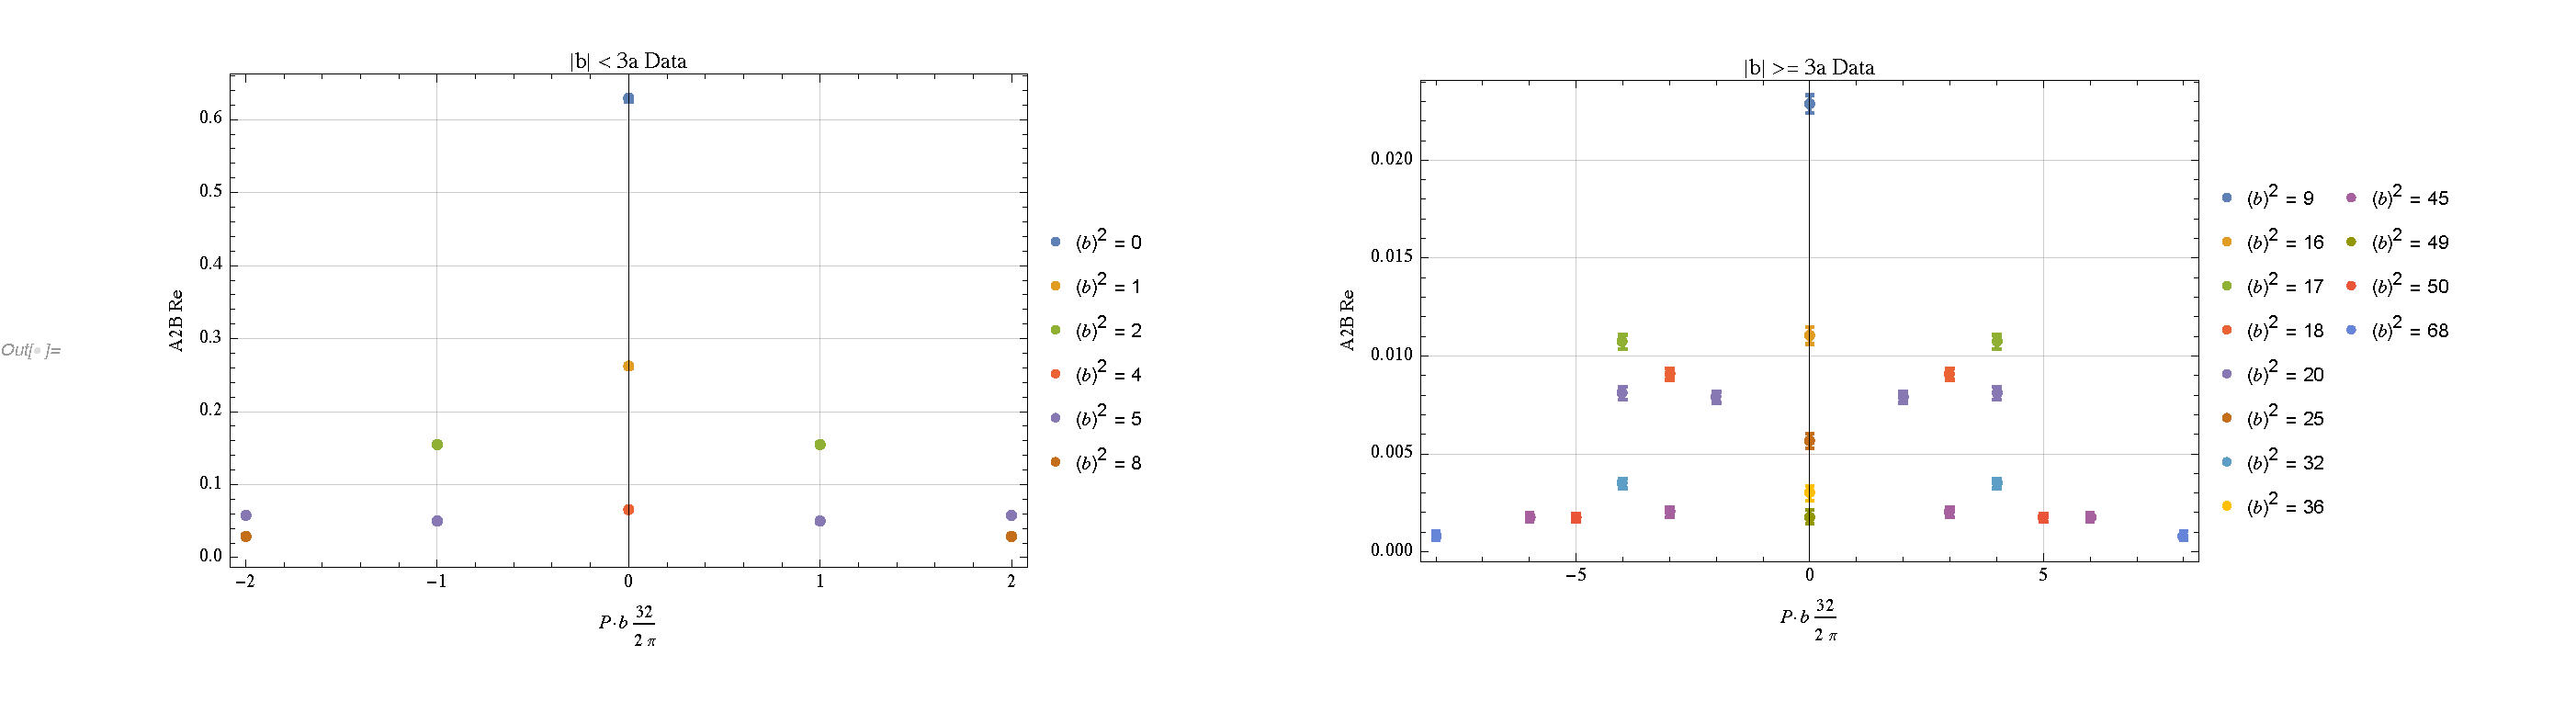
\includegraphics[width=1\linewidth]{plots/short_distance/A2B_Re_b_lessthan3_and_ge3.pdf}
    \caption{Plots of $\tAmp^{Re}_{2B}$ amplitude showing the short-distance data ($|\vect{b}| < 3a$) exhibiting an opposite curvature compared to the long-distance data ($|\vect{b}| \ge 3a$) for fixed momentum ($P=-1$) and fixed $\eta$ (say $\eta=8$)}
\end{figure}

\begin{figure}[H]
    \centering
    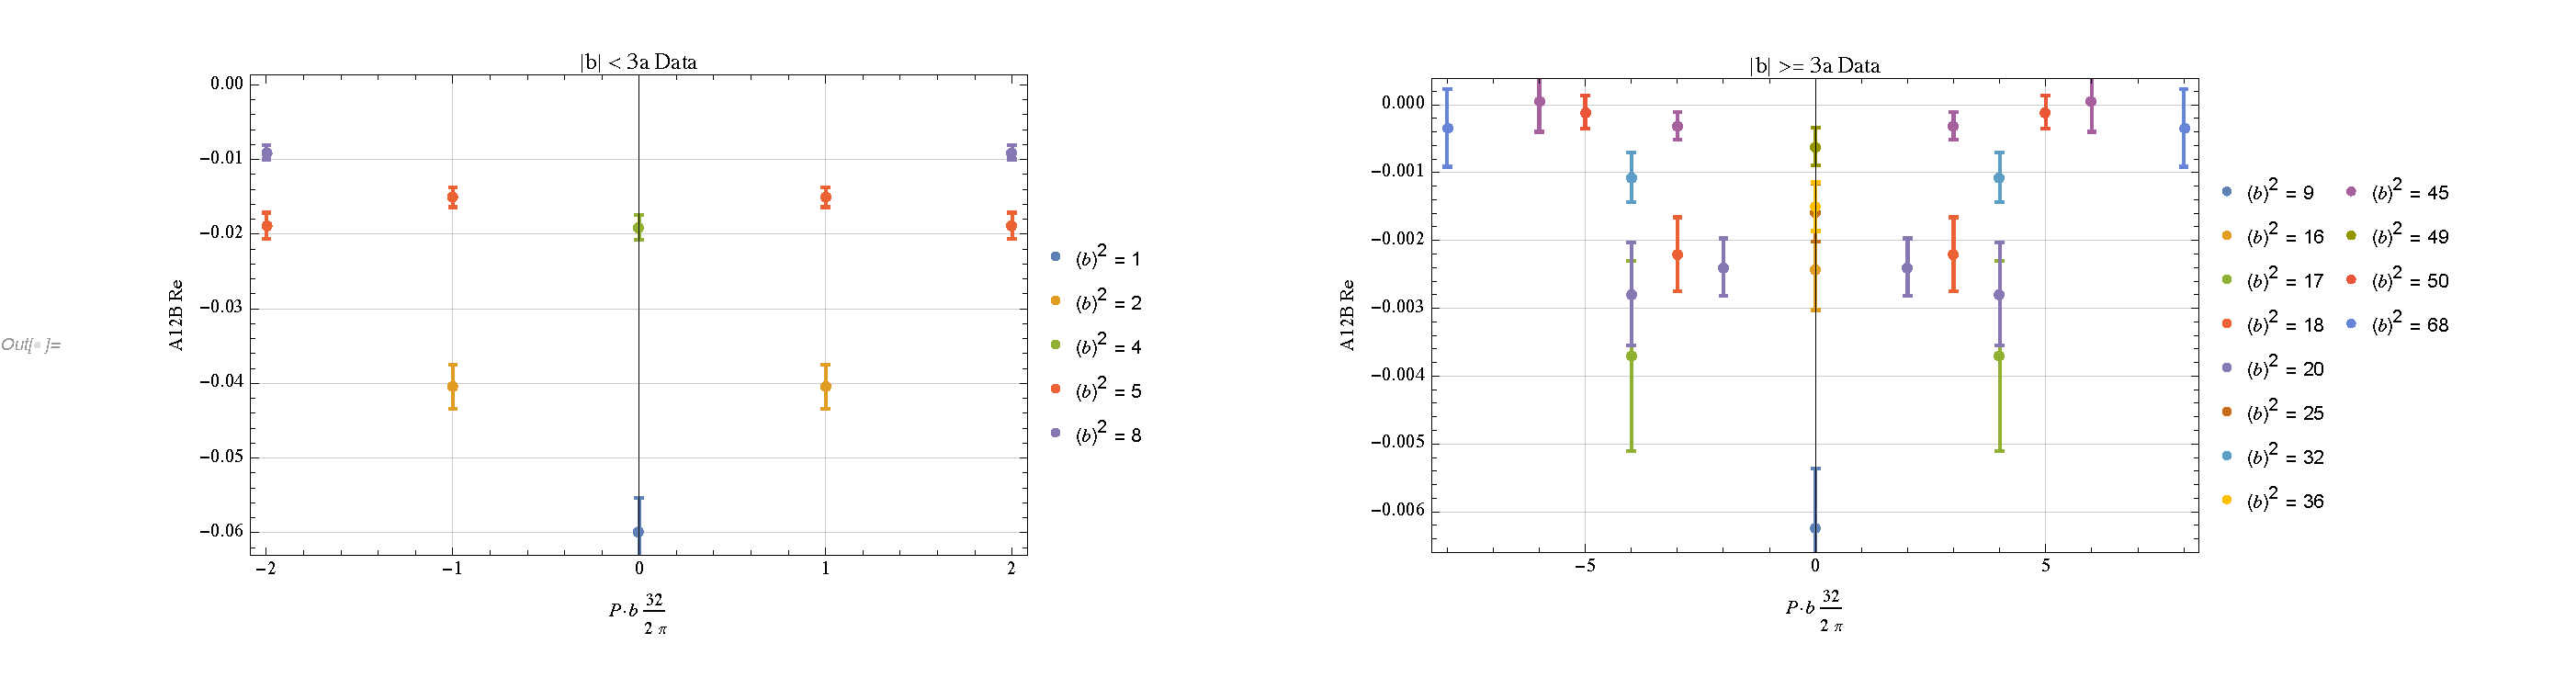
\includegraphics[width=1\linewidth]{plots/short_distance/A12B_Re_b_lessthan3_and_ge3.pdf}
    \caption{Plots of $\tAmp^{Re}_{12B}$ amplitude showing the short-distance data ($|\vect{b}| < 3a$) exhibiting an opposite curvature compared to the long-distance data ($|\vect{b}| \ge 3a$) for fixed momentum ($P=-1$) and fixed $\eta$ (say $\eta=8$)}
\end{figure}

All subsequent stability analyses, global fits, and extracted phenomenological parameters discussed in this chapter are derived strictly from this artifact-suppressed ($|\vect{b}| \ge 3a$) dataset.


\subsection{Physics-Informed Symbolic Regression via PySR}
\label{sec:pysr_methodology}

Selecting a multi-dimensional functional form by hand introduces human bias. To address this, we use Symbolic Regression (SR). 

Unlike traditional regression, which optimizes the parameters of a pre-determined function, symbolic regression searches the space of mathematical expressions and their parameters simultaneously. We utilize \texttt{PySR} \cite{Cranmer2023pysr}, a framework that uses Genetic Programming to discover interpretable equations from data by balancing accuracy and simplicity.

\subsubsection{Expression Search and Configuration}
\texttt{PySR} \cite{Cranmer2023pysr, Koza1992GP, Schmidt2009Distilling} uses a genetic algorithm to evolve mathematical expressions represented as binary trees iteratively. The algorithm evaluates a population of expressions against the lattice data using a custom loss function over thousands of generations. 

Table~\ref {tab: pysr_config} details the \texttt{PySR} search configuration, including the permitted mathematical operators, nesting constraints, and key hyperparameters. The operator library includes a custom Lorentzian-type binary operator, $\text{lor}(x, y) = 1/(1 + x^2 + y^2)^2$, alongside standard arithmetic and exponential functions. At the same time, nesting constraints prevent the algorithm from generating physically meaningless double-exponential or double-decay structures.

\input{PySR_outputs/pysr_model_config}


\subsubsection{The Physics-Informed Custom Loss Function}

Standard symbolic regression optimizes metrics like Mean Squared Error (MSE). However, a genetic algorithm might discover a polynomial or diverging exponential function that fits the finite $(b_L, b_T)$ lattice grid well, but diverges as $b_L \to \infty$. As shown in Section \ref{sec:gaussian_transformation}, this would cause the subsequent Fourier transform over $P \cdot b$ to diverge.

We implemented a custom loss function within \texttt{PySR} to enforce the required asymptotic decay. The reduced chi-squared statistic determines the base accuracy of the model:
\begin{align}
    \mathcal{L}_{\text{base}} = \frac{\chi^2}{\text{dof}} = \frac{1}{N - k} \sum_{i=1}^{N} \left( \frac{\tAmp_{2B}^{\text{Re, lattice}}(i) - \tAmp_{2B}^{\text{Re, model}}(i)}{\sigma_i} \right)^2
\end{align}

Here, $N$ is the number of lattice data points, $k$ is the number of degrees of freedom in the generated expression, and $\sigma_i$ is the statistical error of the $i$-th lattice point.

To enforce the asymptotic decay required for Fourier integrability, we introduce a penalty term. We evaluate the proposed model equation at large values of the longitudinal separation, $b_L^{\text{large}}$, while keeping the transverse separations $b_T$ fixed to physical slices. We compute the sum of the absolute model predictions in this asymptotic regime:
\begin{align}
    \mathcal{P}_{\text{asymptotic}} = \sum_{b_T \in \{b_{T}^{\text{fixed}}\}} \sum_{b_L \in \{b_{L}^{\text{large}}\}} \left| \tAmp_{2B}^{\text{Re, model}}(b_L, b_T) \right|
\end{align}

If a generated equation diverges or grows at large $b_L$, the penalty term $\mathcal{P}_{\text{asymptotic}}$ increases, lowering the equation's fitness score. If the equation decays toward zero, the penalty vanishes.

We combine these terms into the total objective function for \texttt{PySR}. The penalty is scaled by a small regularization parameter $\epsilon$:
\begin{align}
    \mathcal{L}_{\text{custom}} &= \mathcal{L}_{\text{base}} + \epsilon \, \mathcal{P}_{\text{asymptotic}} \\
    \mathcal{L}_{\text{custom}} &= \frac{\chi^2}{\text{dof}} + \epsilon \sum_{b_T \in \{b_{T}^{\text{fixed}}\}} \sum_{b_L \in \{b_{L}^{\text{large}}\}} \left| \tAmp_{2B}^{\text{Re, model}}(b_L, b_T) \right|
\end{align}

By evaluating fitness using $\mathcal{L}_{\text{custom}}$, \texttt{PySR} restricts the search to mathematical expressions that fit the finite lattice data and obey the asymptotic decay constraints. The Julia implementation of this objective function is shown below. The asymptotic penalty evaluates each candidate expression at five test coordinates in the regime $b_L \gg 1$, spanning staple extents $\eta \in \{6, 8, 10\}$ and longitudinal separations up to $b_L = 80a$. We set the regularization weight to $\epsilon = 0.1$.

\input{PySR_outputs/pysr_custom_loss_code}

\subsubsection{Pareto Front of Discovered Models}

Symbolic regression outputs a Pareto front of candidate models: a ranked list of equations that trade off mathematical simplicity (measured by expression tree complexity $C$) and predictive accuracy (measured by the custom loss $\mathcal{L}_{\text{custom}}$). The Pareto front for the real unpolarized amplitude $\tAmp_{2B}^{\text{Re}}$ is presented in Table~\ref{tab:pysr_pareto_front}.

\input{PySR_outputs/pysr_equations_table}

At the lowest complexities ($C \leq 4$), \texttt{PySR} isolates the overall $\eta$-dependence of the amplitude as an exponential decay $\sim (0.499)^\eta \approx e^{-0.695\eta}$, consistent with the area-law suppression of the extended Wilson line. At intermediate complexities ($C = 7$--$12$), the algorithm introduces spatial $b$-dependence through Lorentzian-type power-law denominators $(1 + b_L^2 + b_T^2)^{-j}$ alongside linear or power-law $\eta$-models. The algorithm does not select a Gaussian spatial profile $e^{-cb^2}$ at any point along the Pareto front. It instead converges on the power-law tail structure, aligning with the findings in Section~\ref{sec:gaussian_transformation}.

The models at complexities $C = 14$ and $C = 16$ best balance accuracy and structure. The $C = 14$ expression achieves a factorized form:
\begin{equation}
    \tAmp_{2B}^{\text{Re}} = \frac{39.71}{(1 + b_L^2 + b_T^2)^{1.39}} \, e^{-0.534\eta} \ ,
    \label{eq:pysr_C14}
\end{equation}
which is a product of an exponential decay in $\eta$ and a generalized Lorentzian power-law decay in $b^2 = b_L^2 + b_T^2$. The $C = 16$ model introduces a small additive constant offset of $-0.00127$, reducing the loss to $\mathcal{L}_{\text{custom}} = 2.03$:
\begin{equation}
    \tAmp_{2B}^{\text{Re}} = \frac{245.5}{(1 + b_L^2 + b_T^2)^{1.26}} \, e^{-0.468\eta} - 0.00127 \ .
    \label{eq:pysr_C16}
\end{equation}
Beyond $C = 16$, added complexity yields marginal loss improvements while reducing interpretability.

The power-law tail $(1 + b^2)^{-j}$ with $j > 1/2$ decays algebraically at large separations. This decays more slowly than a Gaussian but remains absolutely integrable over the real line. Unlike the Gaussian model, where the sign of $(\alpha - \beta)$ can render the Fourier integral divergent, the power-law denominator guarantees convergent integrals for positive exponents $j > 1/2$. The factorized structure $e^{-f\eta} \times g(b^2)$ also allows the shared $\eta$-dependent exponential to cancel analytically in the Sivers shift ratio, which we use in Section~\ref{sec:simultaneous_fit_strategy}.

\begin{figure}[htbp]
    \centering
    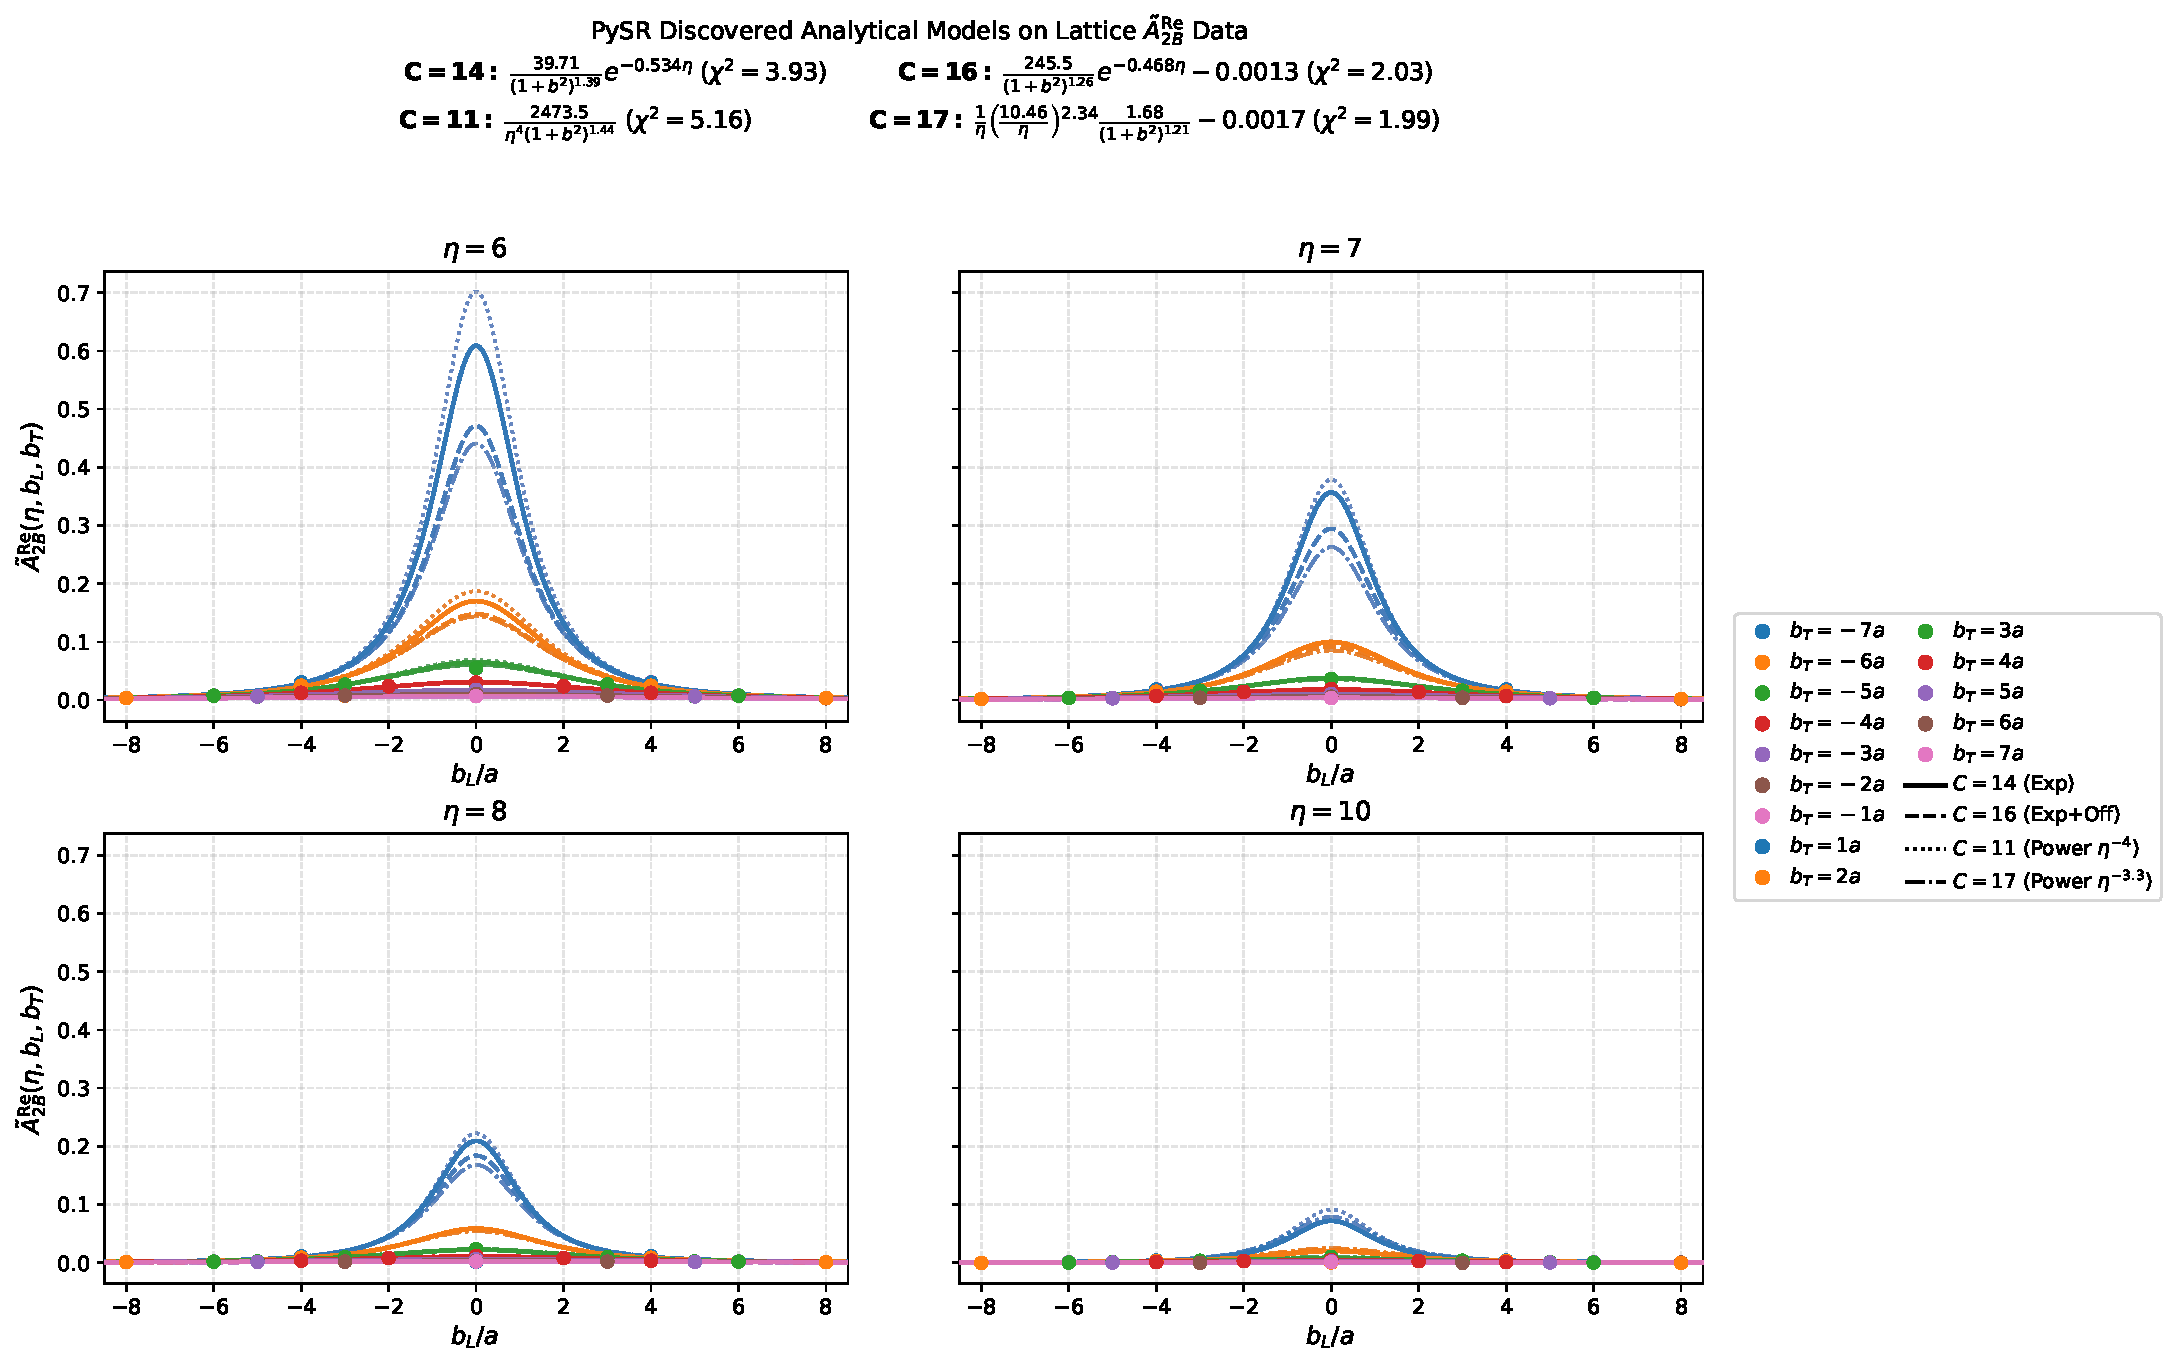
\includegraphics[width=1\linewidth]{PySR_outputs/01_A2B_PySR_Benchmark_Fits.pdf}
    \caption{Multi-panel comparison of the top \texttt{PySR}-discovered analytical models ($C = 11, 14, 16, 17$) against the lattice data for $\tAmp_{2B}^{\text{Re}}$ at fixed staple extents $\eta = 6, 7, 8, 10$ (with $P_1 = -1$ and $|\vect{b}| \geq 3a$). Each panel displays the amplitude as a function of the longitudinal separation $b_L/a$ at fixed transverse separations $b_T$, with the four Pareto-front models overlaid. The two exponential-$\eta$ models ($C = 14$, solid; $C = 16$, dashed) provide the most balanced description across all $\eta$ values, while the pure power-law-$\eta$ models ($C = 11$, dotted; $C = 17$, dot-dashed) exhibit slight systematic deviations at the extremes of the $\eta$ range.}
    \label{fig:pysr_benchmark_fits}
\end{figure}

\begin{figure}[htbp]
    \centering
    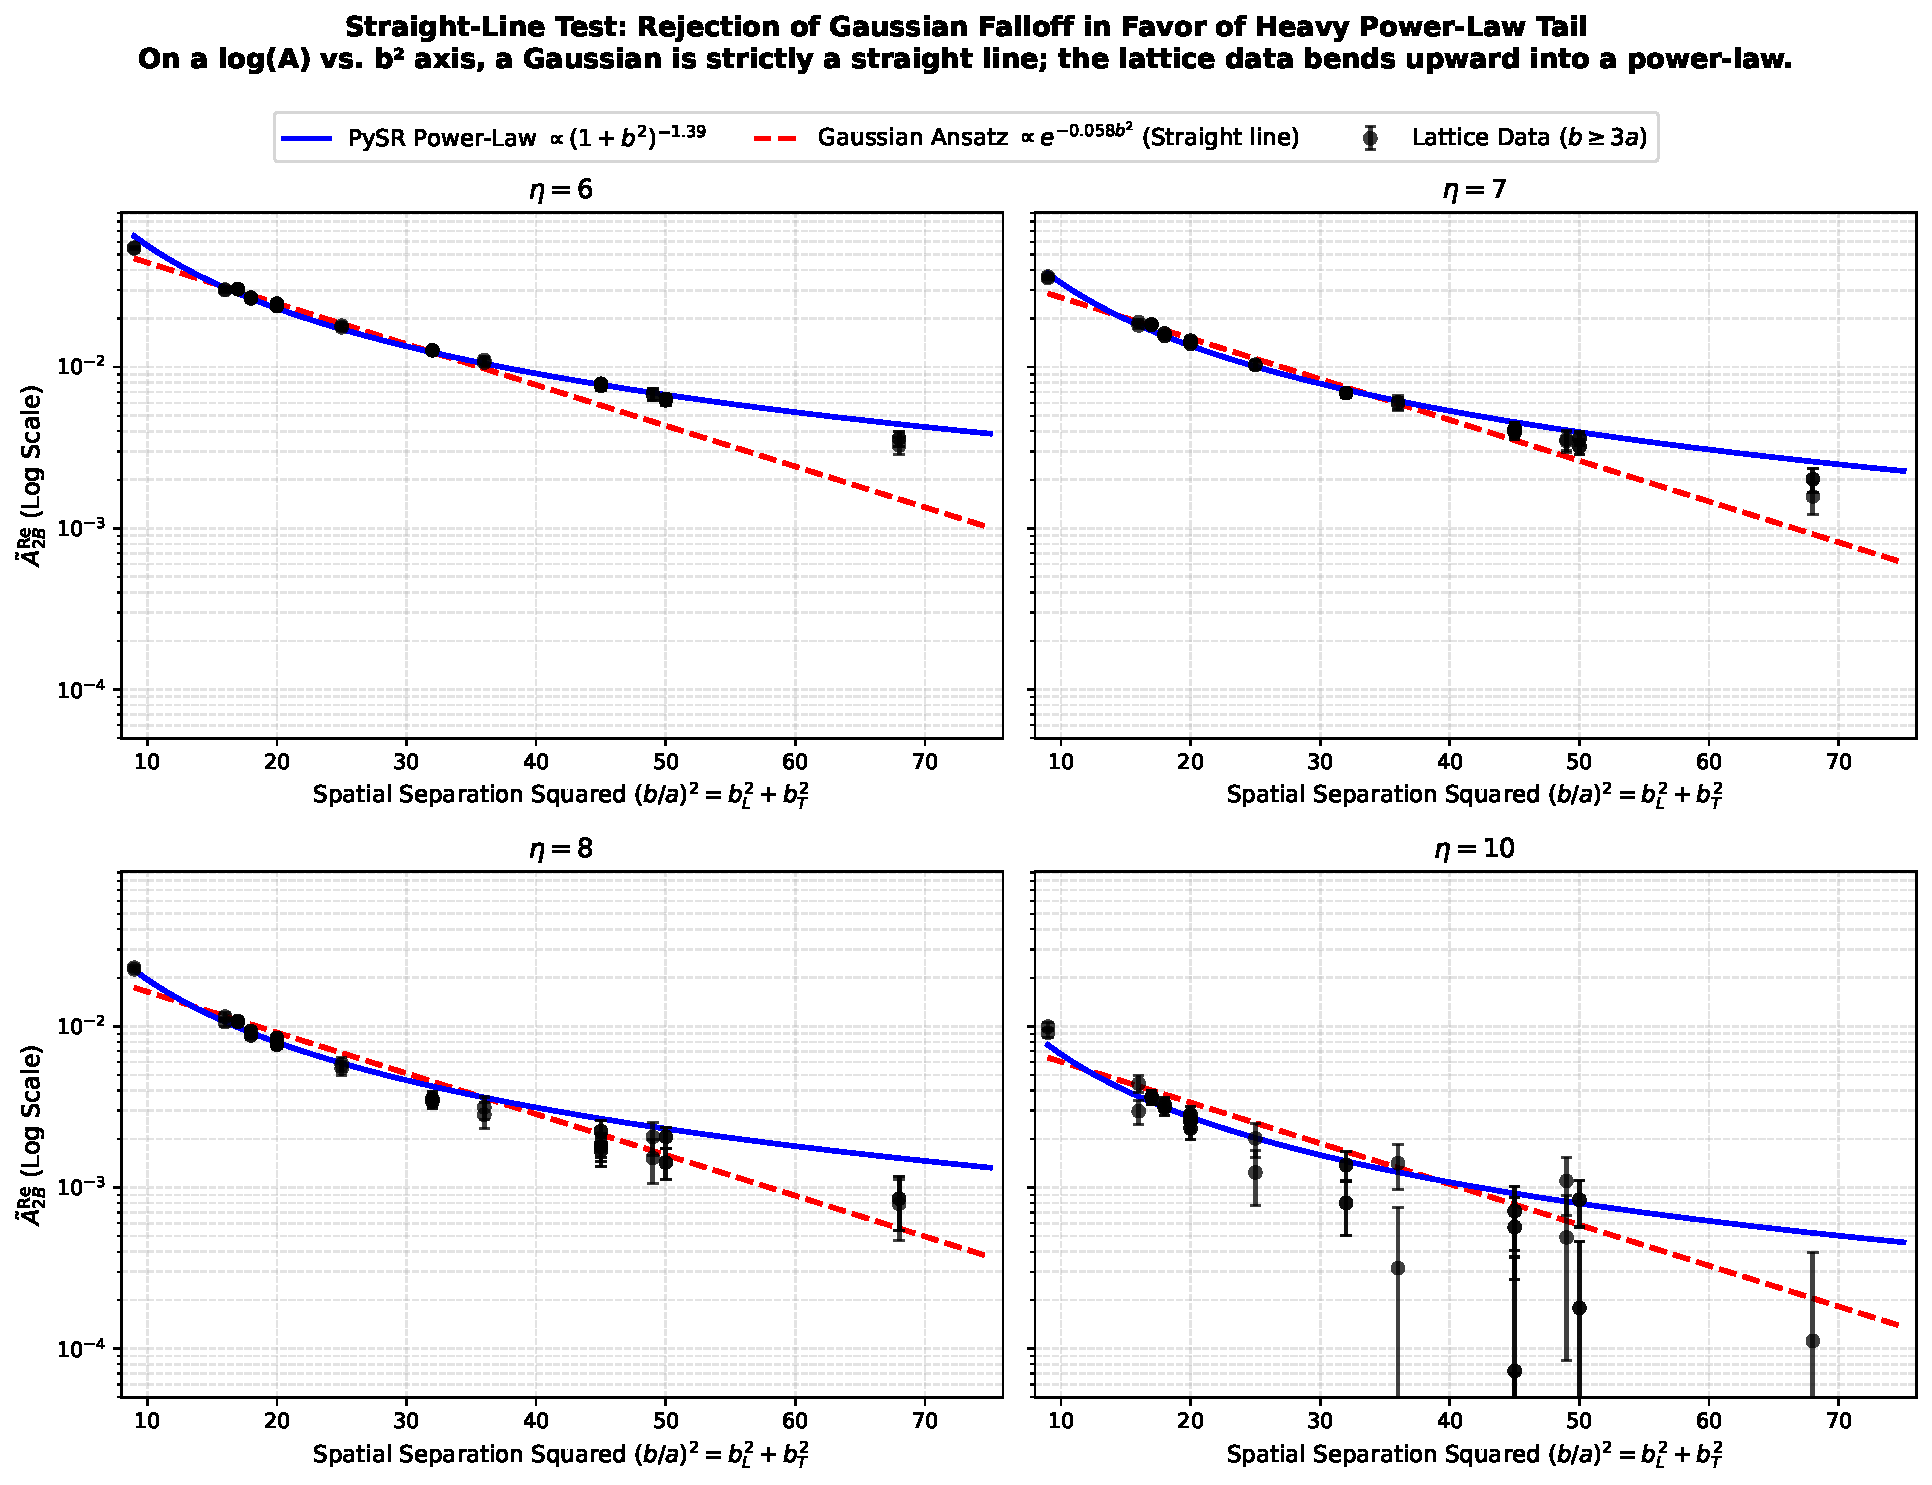
\includegraphics[width=0.95\linewidth]{PySR_outputs/02_Gaussian_StraightLine_Test.pdf}
    \caption{Diagnostic straight-line test for the Gaussian hypothesis. If the amplitude followed a pure Gaussian profile $\tAmp_{2B}^{\text{Re}} \propto e^{-c\,b^2}$, the data would appear as a straight line on a logarithmic ordinate versus $b^2$ (red dashed line, optimal Gaussian fit with $c = 0.058$). The lattice data (black markers) exhibit clear upward curvature away from the Gaussian baseline at large $b^2$, indicating a heavier-than-Gaussian tail that is accurately captured by the \texttt{PySR}-discovered power-law form $(1 + b^2)^{-1.39}$ (blue solid line). This provides direct, model-independent evidence that the spatial decay of the non-local quark bilinear follows an algebraic power law rather than a Gaussian exponential.}
    \label{fig:gaussian_straightline_test}
\end{figure}

As shown in Fig.~\ref{fig:pysr_benchmark_fits}, the factorized $C = 14$ and $C = 16$ expressions track the lattice data throughout the accessible $(b_L, b_T)$ grid across all staple extents. The pure power-law-$\eta$ models ($C = 11, 17$) exhibit slight systematic tension at the boundary $\eta$ values, where their $\eta^{-n}$ dependence departs from the exponential decay.

The straight-line diagnostic in Fig.~\ref{fig:gaussian_straightline_test} tests the Gaussian hypothesis. If the amplitude followed a Gaussian decay, plotting $\tAmp_{2B}^{\text{Re}}$ on a logarithmic ordinate against $b^2$ would yield a straight line with slope $-c$. The lattice data shows upward curvature at large $b^2$, indicating that the amplitude decays more slowly than an exponential. This behavior matches the generalized Lorentzian power-law tail discovered by the genetic algorithm.

Based on these results, we adopt the Lorentzian power-law structure as the spatial profile for $\tAmp_{2B}^{\text{Re}}$. In the following sections, we extend this functional form to the remaining amplitudes for the global simultaneous fit.

\subsection{Test for Factorization in $(P\cdot b)$ and $b^2$} \label{Test-for-Factorization}

To probe, directly at the level of the raw lattice data and independent of any fitted parameterization, whether the extracted amplitude factorizes as $\tAmp(P\cdot b,b^2) = F(P\cdot b) G(b^2)$, we performed a ratio test at fixed $P\cdot b$, which has multiple $b^2$, for example $b^2_1,b^2_2, b^2_3$, at the given momentum $P_L$. We formed
$$
R(b^2_i) = \frac{\tAmp(P\cdot b, b^2_i)}{\tAmp(P\cdot b, b^2_3)}
$$

\begin{figure}[htbp]
    \centering
    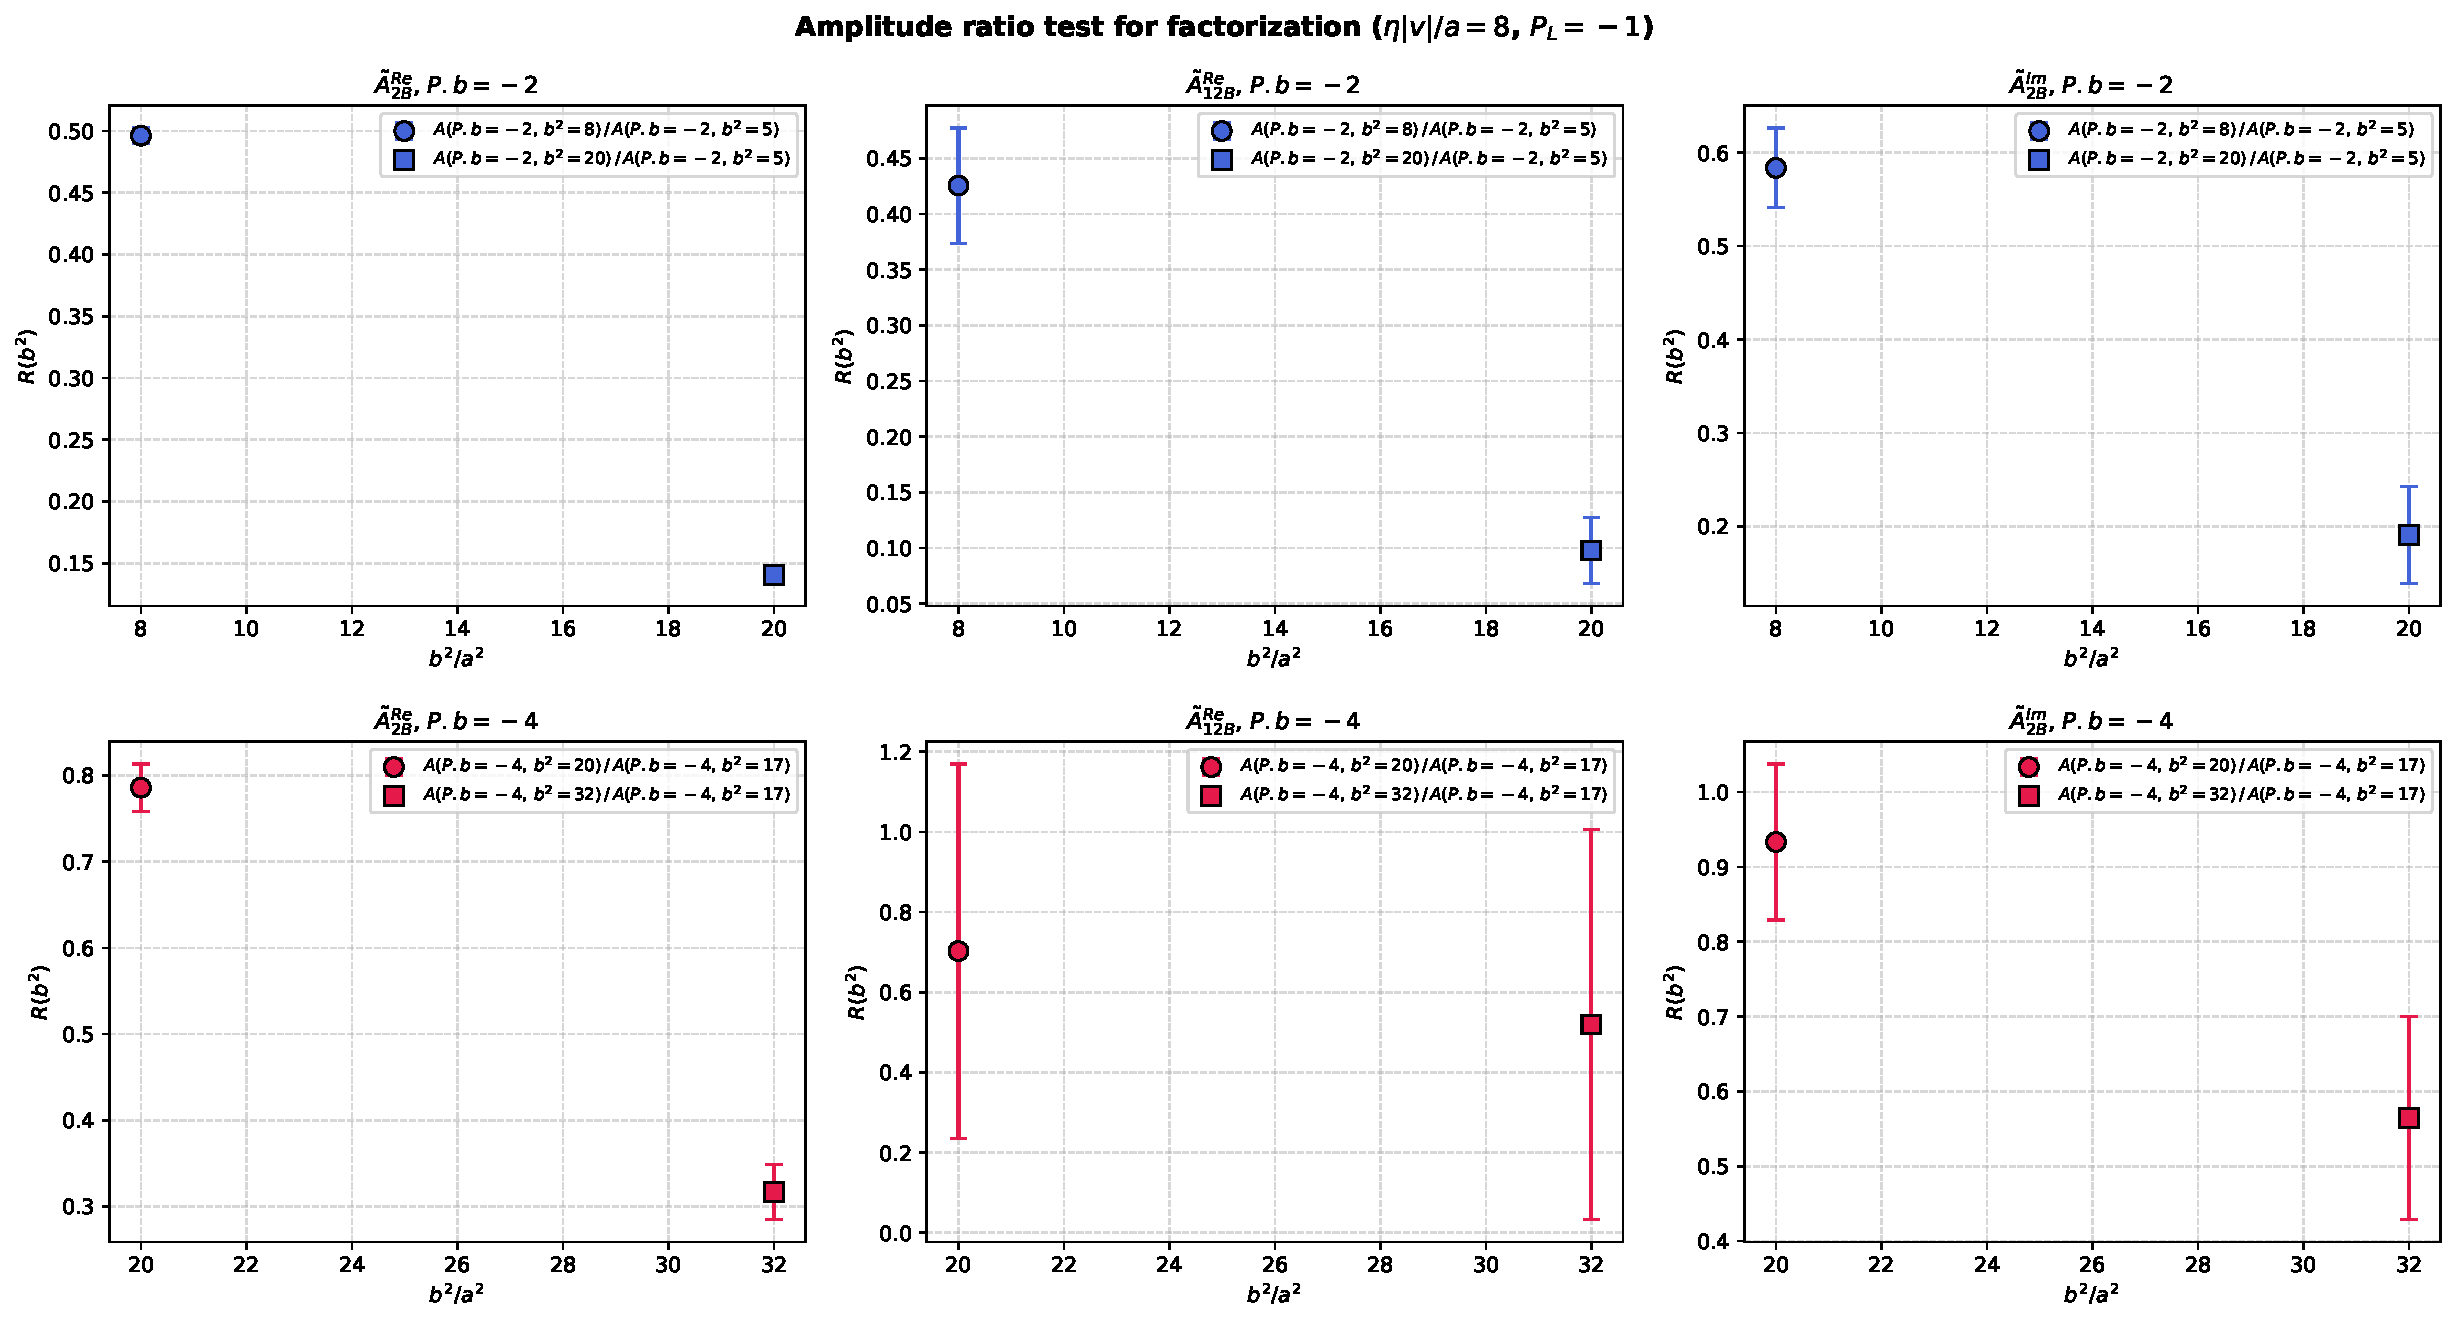
\includegraphics[width=1\linewidth]{plots/FixedPb_Bsq_RatioTest_eta8_PL-1.pdf}
    \caption{Ratio test for $(P\cdot b,b^2)$ factorization at fixed $P\cdot b$, for $\tAmp_{2B}^{\rm Re}$, $\tAmp_{12B}^{\rm Re}$, and $\tAmp_{2B}^{\rm Im}$ at $\eta|v|/a=8$, $P_L=-1$. Top row: $P\cdot b=-2$; bottom row: $P\cdot b=-4$; each point is ratioed against that row's own smallest available $b^2$, with the explicit ratio given in the legend.}
    \label{fig:FixedPb_Bsq_RatioTest_eta8_PL-1}
\end{figure}

The two rows in Fig.~\ref{fig:FixedPb_Bsq_RatioTest_eta8_PL-1} do not trace a common zero-slope line in $b^2$, as a factorized ansatz would predict. A fully model-independent version of this test would additionally require ratioing at fixed $b^2$ between different values of $P\cdot b$; however, the $(b_L,b_T)$ points computed on the lattice do not form a regular grid in $(P\cdot b,b^2)$, and at most two distinct $P\cdot b$ values ever coincide at a common $b^2$ anywhere in the dataset, with no two $P\cdot b$ rows sharing two or more common $b^2$ values. This limited sampling prevents us from carrying out the complementary ratio test at fixed $b^2$. Given this limitation, while the data appears to disfavor an exactly factorized ansatz, we treat this observation only as a qualitative guide rather than a firm conclusion. In the next section, we instead explore a fit model built directly on a factorized ansatz along with several non-factorized ansatze.



\subsection{Systematical exploration of the best physical model}
Based on the \texttt{PySR} analysis, we started exploring numerous power-law models for $\tAmp_{2B}^{\text{Re}}$ for momentum $P_L=-1$, $6\leq\eta\leq10$, and $b\geq3$. For completeness, we started with a Gaussian model and introduced several $\eta$-dependent ans\"atzes. For each model, the table lists the model expression, the list of fit parameters, the jackknife-averaged fitted values with statistical uncertainties, and the resulting $\chi^2/\mathrm{DoF}$.
\begin{figure}[htbp]
    \centering
    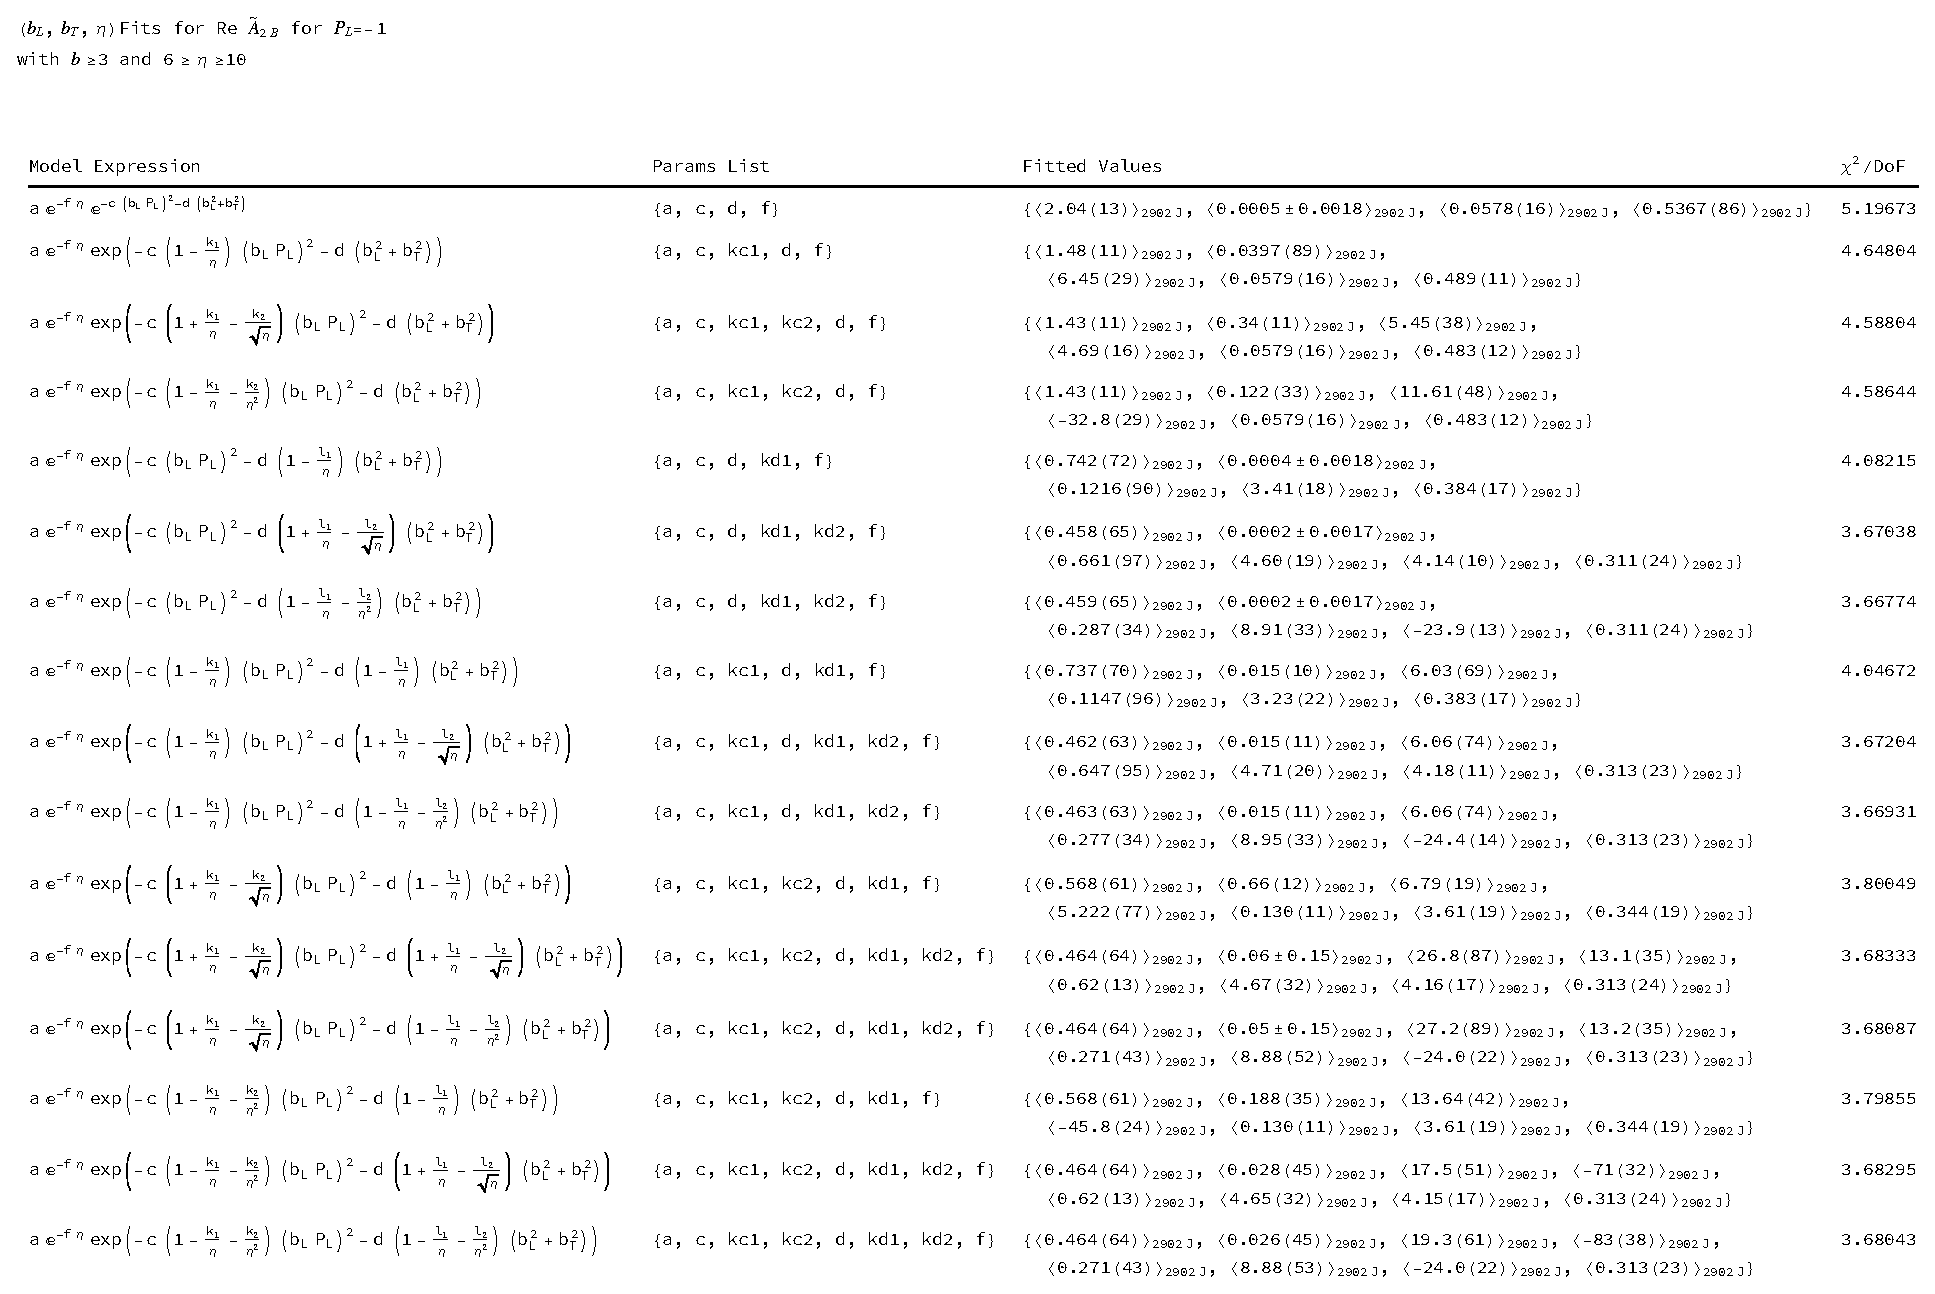
\includegraphics[width=0.8\linewidth]{plots/fit_exploration_mathematica/fit_list_gaussian_c_d_etas.eps}
    \caption{3D jackknife fits of $\mathrm{Re}\,\tilde{A}_{2B}(b_L,b_T,\eta)$ to a family of 16 Gaussian ans\"atze, all built on the common baseline $\tilde{A}_{2B} = a\, e^{-f\eta}\, \exp\!\big[-c\,(b_L P_L)^2 - d\,(b_L^2+b_T^2)\big]$, in which the coefficients $c$ and $d$ are each independently allowed to be either constant or one of three $\eta$-dependent forms, $c\to c(\eta)$ and/or $d\to d(\eta)$.}
    \label{fig:rejection_fit_list_gaussian_c_d_etas}
\end{figure}

From our physics requirements, we strictly want the fit parameter $c$ to be positive and statistically stable, because $c$ is the coefficient of $P.b$, and having a stable, positive $c$ is needed for a physical Fourier-transformed space in $x$. From Figure \ref{fig:rejection_fit_list_gaussian_c_d_etas}, most $c$ parameters are either unstable or negative, and everything still has a higher $\chi^2/\mathrm{DoF}$. On exploring power-law ans\"atze for for $\tAmp_{2B}^{\text{Re}}$ for momentum $P_L=-1$, $6\leq\eta\leq10$, and $b\geq3$, we could able to further reduce the $\chi^2/\mathrm{DoF}$ $\approx1.5$. We found that $\eta$-dependence in the fit parameter $d$ worsens the fit, while $\eta$-dependence in the fit parameter $c$ improves it. New ambiguity arises: there exist multiple $\eta$ dependencies that all give consistently the same $\chi^2/\mathrm{DoF}$. For each power-law model, the table lists the model expression, the list of fit parameters, the jackknife-averaged fitted values with statistical uncertainties, $\chi^2/\mathrm{DoF}$, AIC, and the resulting Fourier transform in $x$ space.
\begin{figure}[h!]
    \centering
    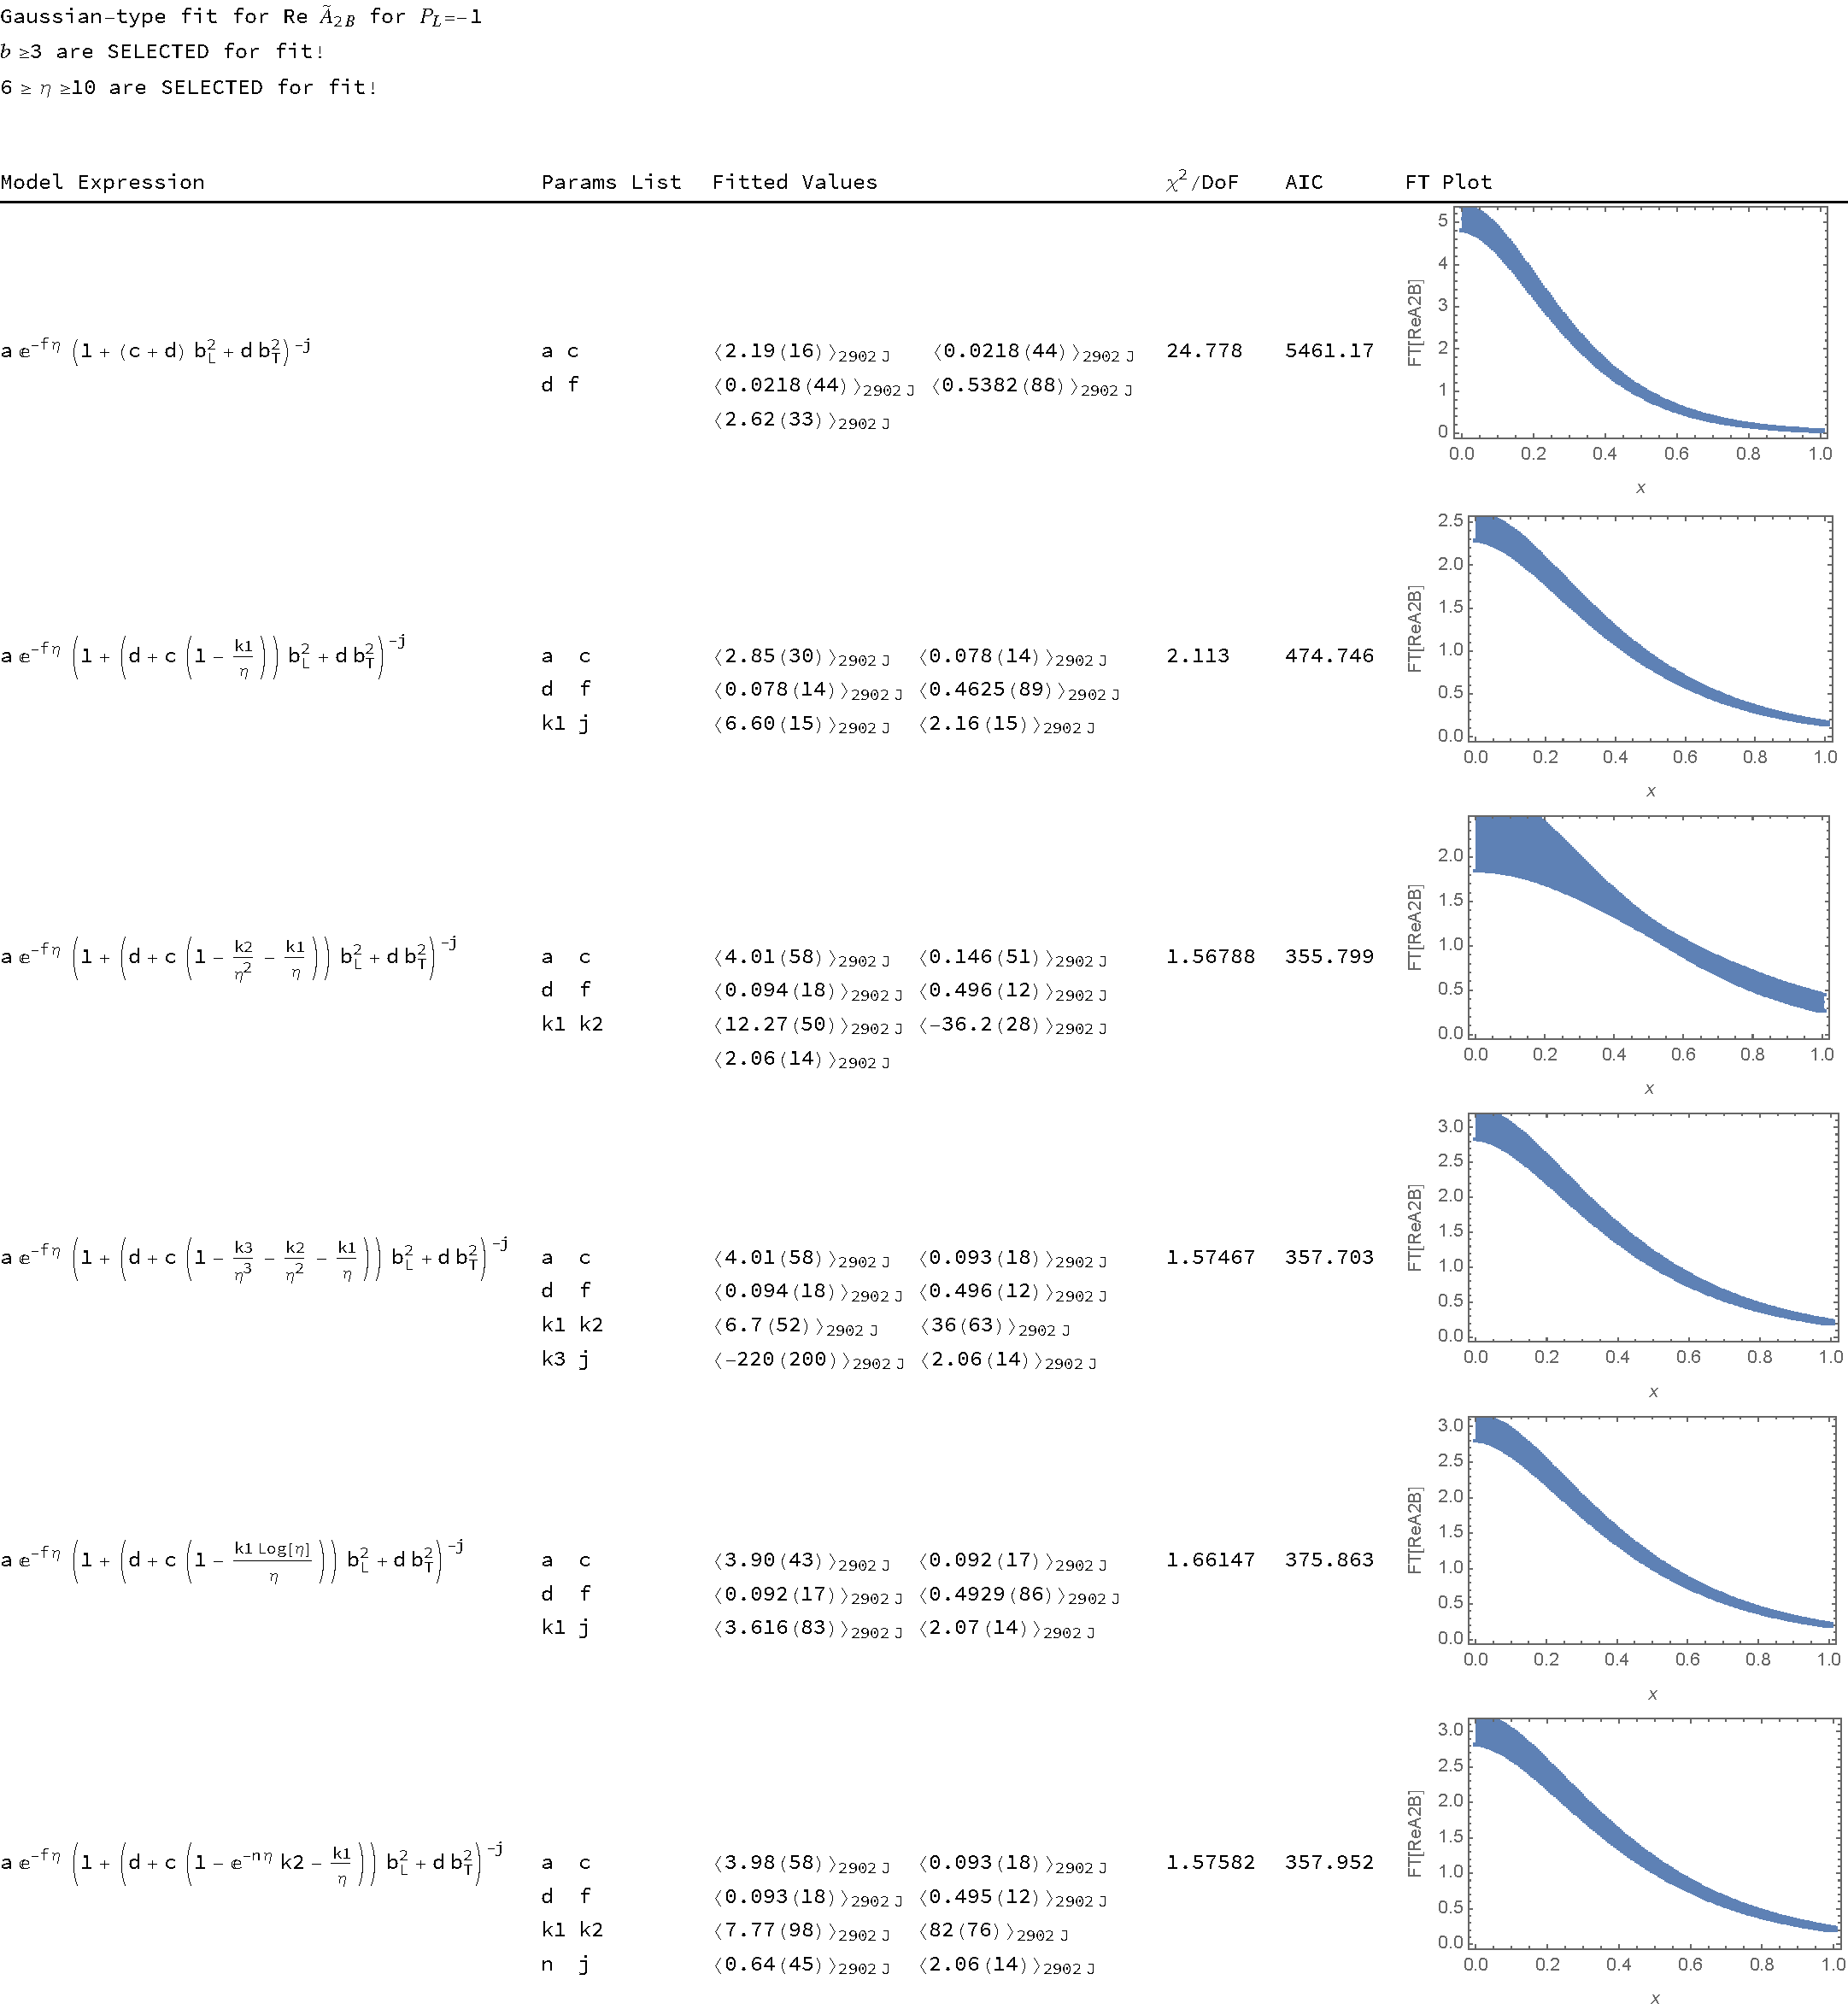
\includegraphics[width=0.8\linewidth]{PowerLaw_etaAsymptotic/A2BfitFT_eta_Asymptotic_P1.pdf}
    \caption{3D Jackknife fits of $\mathrm{Re}\,\tilde{A}_{2B}(b_L,b_T,\eta)$ to a family of power-law ans\"atze, all built on the common baseline $\tilde{A}_{2B} = a\, e^{-f\eta}\, \left(1+(c+d)b^2_L+db^2_T\right)^j$, in which the coefficient $c$ is each independently allowed to be either constant or one of $\eta$-dependent forms, $c\to c(\eta)$.}
\end{figure}
\pagebreak

For completeness, we explored more $\eta$-dependent forms $c\to c(\eta)$, which yield wider Fourier transforms in $x$ space.
\begin{figure}[h!]
    \centering
    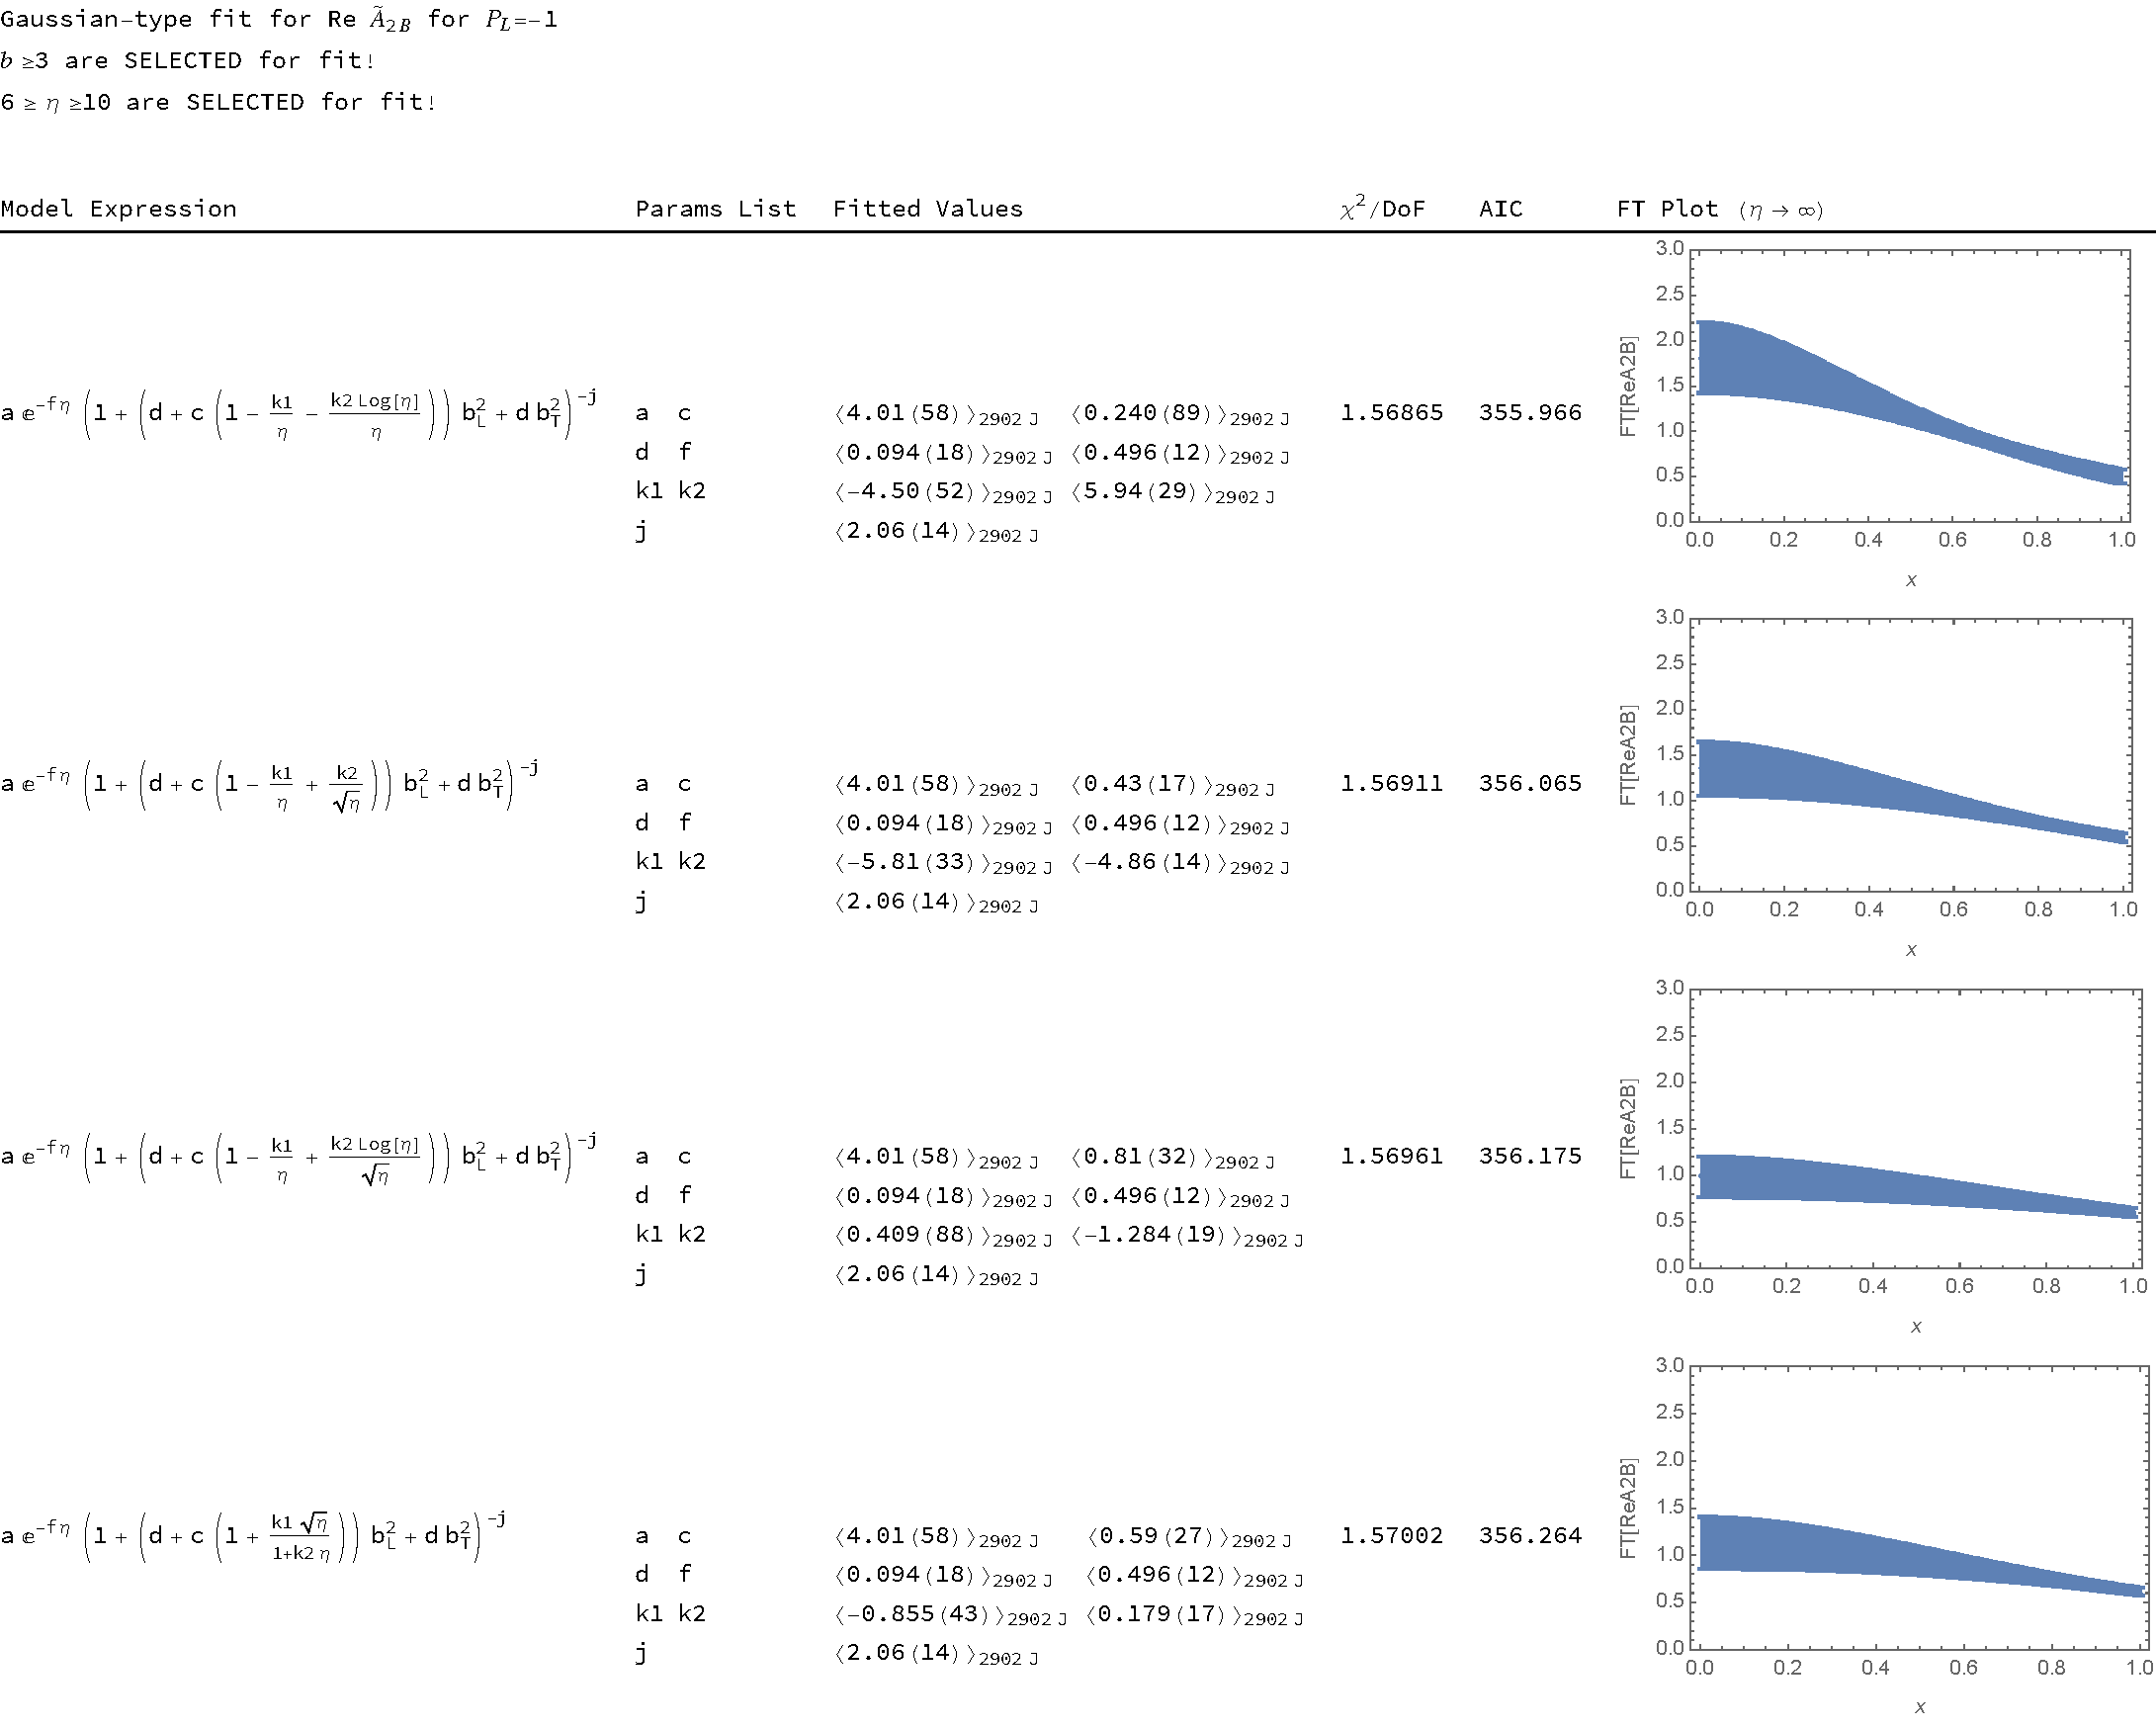
\includegraphics[width=0.8\linewidth]{PowerLaw_etaAsymptotic/A2Bfit_widerFT_eta_Asymptotic_P1.pdf}
    \caption{3D jackknife fits of $\mathrm{Re}\,\tilde{A}_{2B}(b_L,b_T,\eta)$ to a family of power-law ans\"atze, all built on the common baseline $\tilde{A}_{2B} = a\, e^{-f\eta}\, \left(1+(c+d)b^2_L+db^2_T\right)^j$, in which the coefficient $c$ is each independently allowed to $\eta$-dependent forms, $c\to c(\eta)$ which yield wider Fourier transforms in $x$ space.}
\end{figure}

All viable asymptotic functions in $\eta$ have a common power-law profile with a power $j \approx 2$ and an amplitude scale $a \approx 4$, damped by the area-law-like suppression factor $e^{-0.5\eta}$. We isolate the specific $\eta$-dependence of the width parameters $c$ and $d$ by fixing these structural parameters ($j=2$, $a=4$) and performing sequential fits at individual $\eta$ slices. The results are shown below:
\pagebreak
\begin{figure}[htbp]
    \centering
    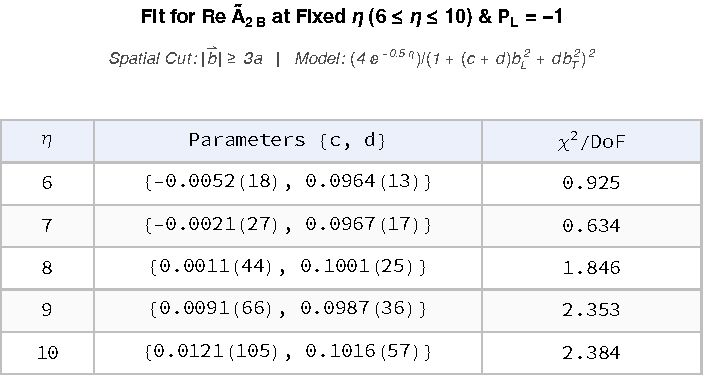
\includegraphics[width=0.6\linewidth]{Gaussian_type_fit_Real_A2B/LorentzianFixedA_P-1_b3.pdf}
    \caption{Sequential Lorentzian fits for $\tAmp^{Re}_{2B}$ at individual $\eta$ slices, holding the global power $j=2$ and amplitude $a=4$ constant.}
    \label{fig:ReA2B_fixed_eta_slices}
\end{figure}

From these fits, we extract the parameters $c$ and $d$. The fit parameter $c$ acts as a coefficient of the longitudinal separation $(P \cdot b)$, while $d$ acts as a coefficient of the invariant squared separation $b^2$. We plot the extracted values of $c$ and $d$ against our candidate asymptotic models to analyze their $\eta$-dependence:

\begin{figure}[h!]
    \centering
    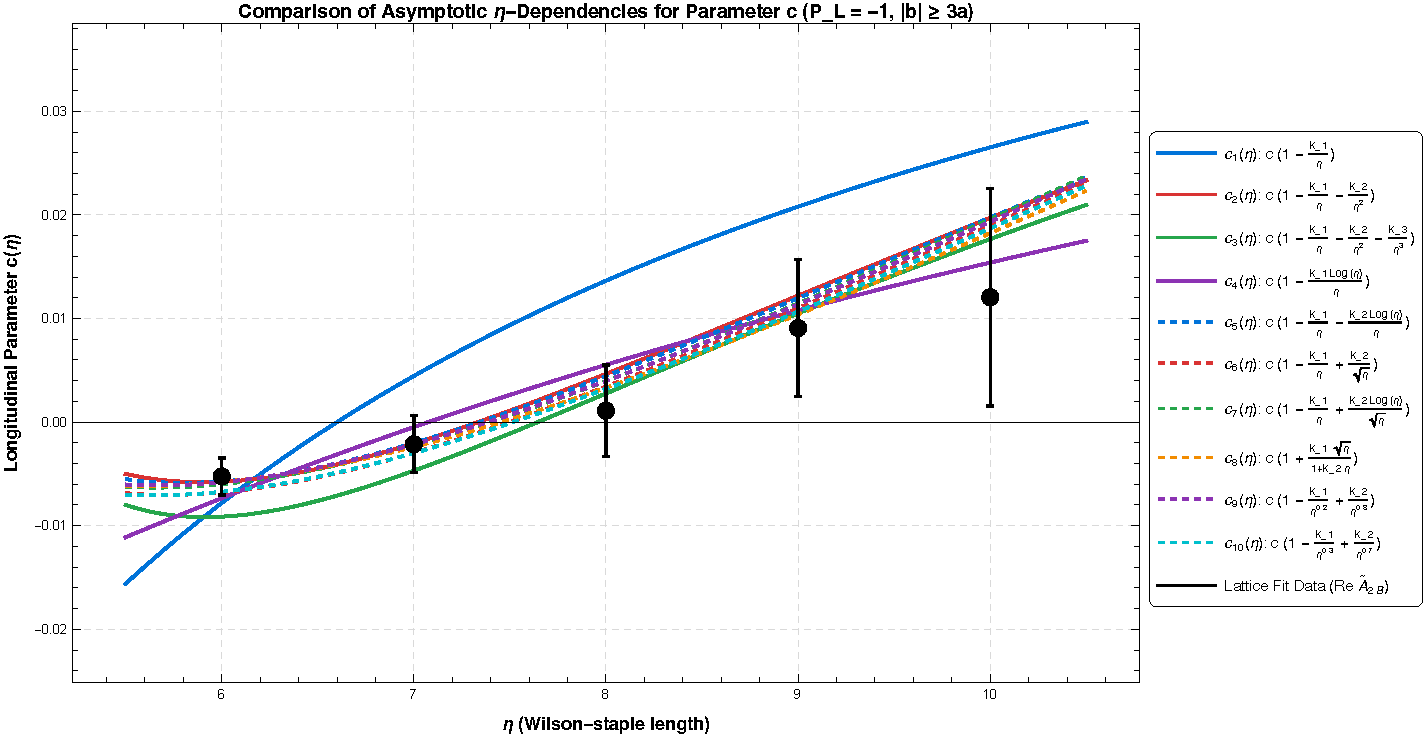
\includegraphics[width=0.5\linewidth]{PowerLaw_etaAsymptotic/A2B_c_eta_AllAsymptoticModels_P1.pdf}
    \caption{The extracted parameter $c(\eta)$ overlaid with various candidate asymptotic models, demonstrating its asymptotic approach at large $\eta$.}
\end{figure}

\begin{figure}[h!]
    \centering
    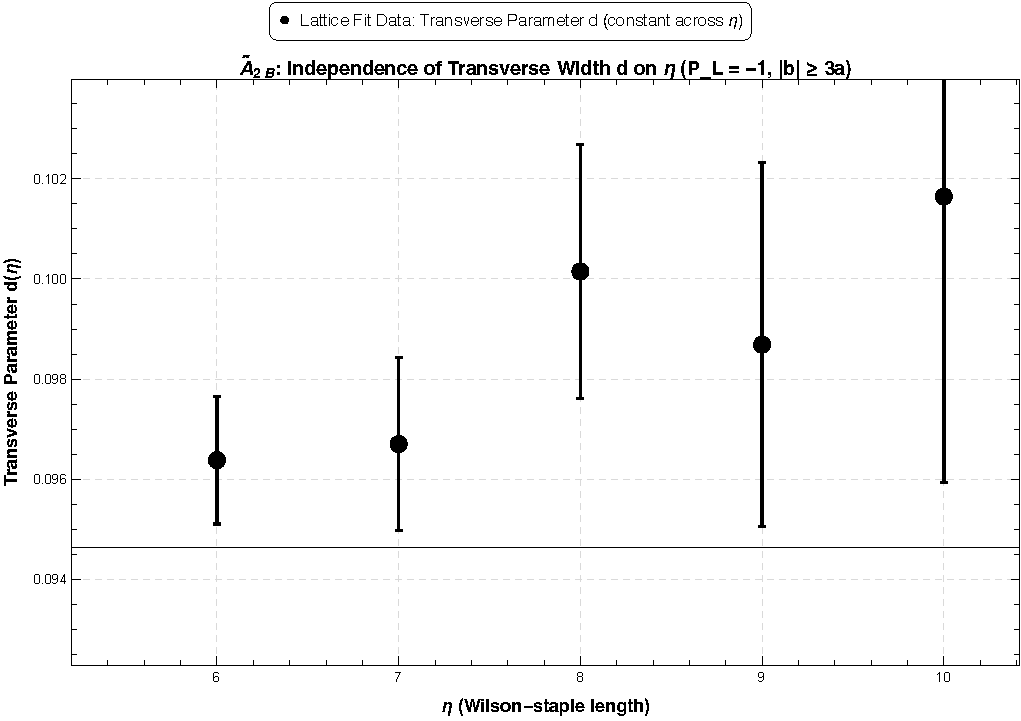
\includegraphics[width=0.4\linewidth]{PowerLaw_etaAsymptotic/A2B_d_eta_Independence_P1.pdf}
    \caption{The extracted parameter $d(\eta)$, exhibiting a clear independence from the staple extent $\eta$.}
\end{figure}


\subsection{Candidate Selection}
\label{sec:candidate_selection}

Based on the $\chi^2/\text{dof}$ minimizations and sequential fitting at individual $\eta$ slices, we determined the structural parameterizations for the invariant amplitudes: $\tAmp_{2B}^{\text{Re}}$, $\tAmp_{2B}^{\text{Im}}$, and $\tAmp_{12B}^{\text{Re}}$. We exclude $\tAmp_{12B}^{\text{Im}}$ because the lattice data is consistent with zero.

For the unpolarized real amplitude $\tAmp_{2B}^{\text{Re}}$, the transverse width parameter $d$ remains constant across all $\eta$, but the longitudinal width parameter $c(\eta)$ requires an asymptotic model. We select the model $c(\eta) = c\left(1 - \frac{k_1}{\eta} - \frac{k_2}{\eta^2}\right)$ because its Fourier transform suppresses negative-$x$ contributions, which we discuss in later sections.

For the real Sivers amplitude $\tAmp_{12B}^{\text{Re}}$, we repeated the sequential Lorentzian fitting at fixed $\eta$ slices. As shown in Fig.~\ref{fig:ReA12B_eta_independence} and Table \ref{tab:ReA12B_fixed_eta}, the longitudinal parameter $c$ and transverse parameter $d$ are independent of $\eta$. We therefore model $c$ and $d$ as constants for $\tAmp_{12B}^{\text{Re}}$.

\begin{table}[h!]
    \centering
    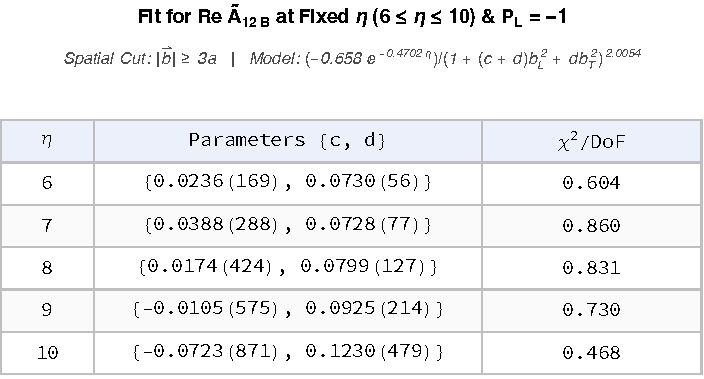
\includegraphics[width=0.55\linewidth]{Gaussian_type_fit_Real_A2B/LorentzianFixed_ReA12B_P-1_b3.pdf}
    \caption{Sequential Lorentzian fits for $\tAmp_{12B}^{\text{Re}}$ at individual $\eta$ slices showing consistent $\chi^2/\text{dof}$ and stable parameters.}
    \label{tab:ReA12B_fixed_eta}
\end{table}

\begin{figure}[h!]
    \centering
    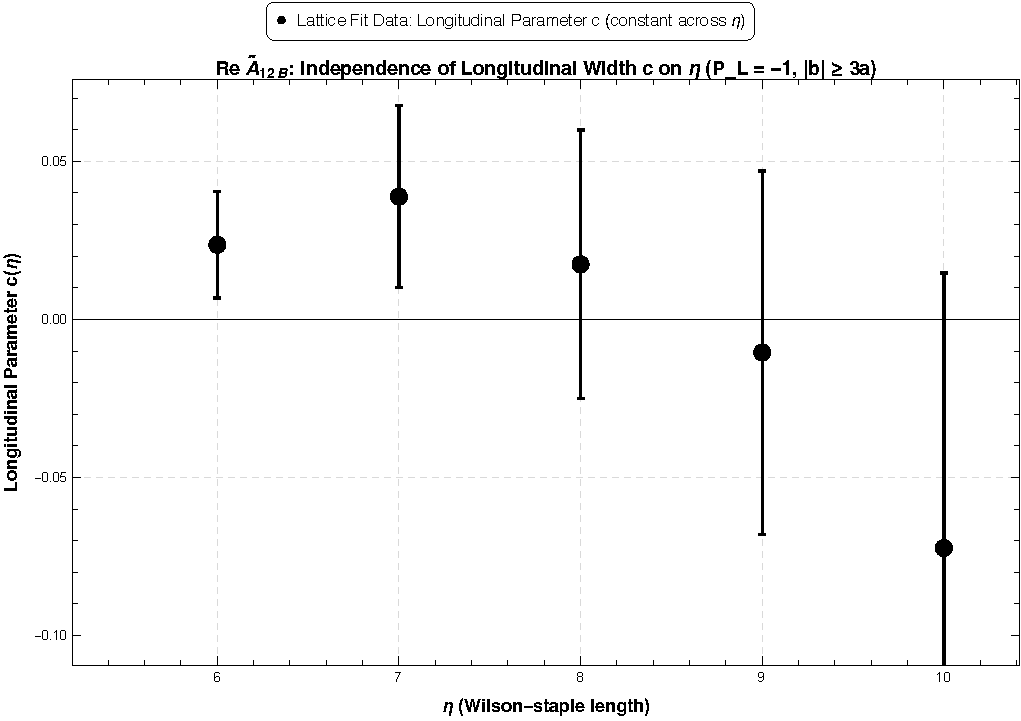
\includegraphics[width=0.49\linewidth]{PowerLaw_etaAsymptotic/ReA12B_c_eta_Independence_P1.pdf}
    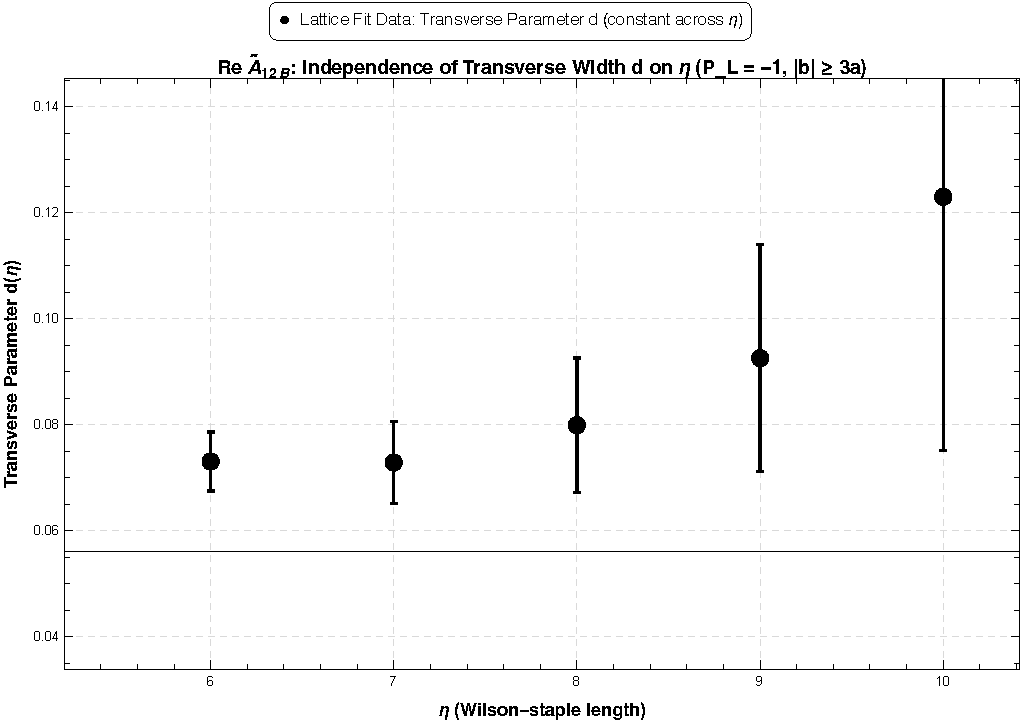
\includegraphics[width=0.49\linewidth]{PowerLaw_etaAsymptotic/ReA12B_d_eta_Independence_P1.pdf}
    \caption{Lattice extracted parameters $c$ (left) and $d$ (right) for $\tAmp_{12B}^{\text{Re}}$ as a function of $\eta$. Both parameters demonstrate clear independence from $\eta$.}
    \label{fig:ReA12B_eta_independence}
\end{figure}

For the imaginary unpolarized amplitude $\tAmp_{2B}^{\text{Im}}$, the lattice data has more statistical noise, but the sequential fitting yields a similar trend. We model $c$ and $d$ as constant in $\eta$, mirroring the structural stability of the real amplitudes. The resulting fits are shown in Fig.~\ref{fig:ImA2B_eta_independence} and Table \ref{tab:ImA2B_fixed_eta}.

\begin{table}[h!]
    \centering
    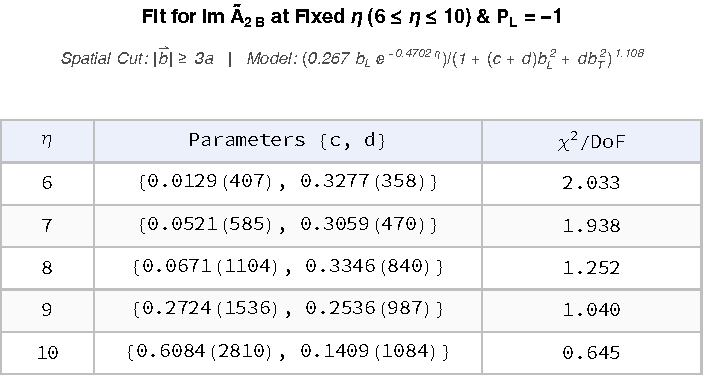
\includegraphics[width=0.55\linewidth]{Gaussian_type_fit_Real_A2B/LorentzianFixed_ImA2B_P-1_b3.pdf}
    \caption{Sequential Lorentzian fits for $\tAmp_{2B}^{\text{Im}}$ at individual $\eta$ slices showing consistent $\chi^2/\text{dof}$.}
    \label{tab:ImA2B_fixed_eta}
\end{table}

\begin{figure}[h!]
    \centering
    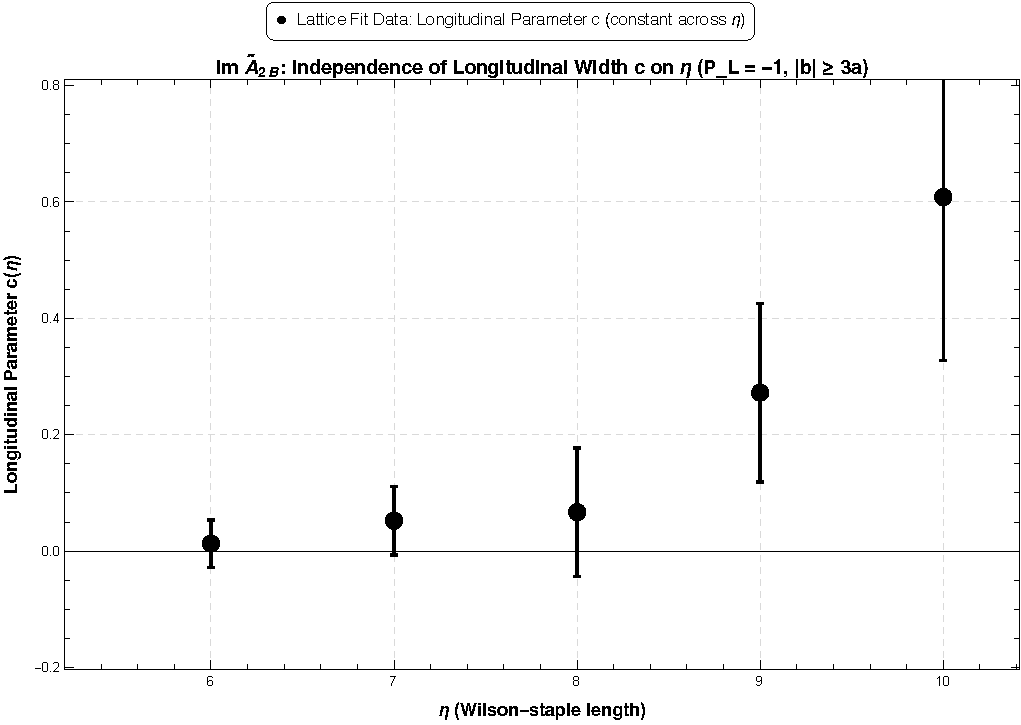
\includegraphics[width=0.49\linewidth]{PowerLaw_etaAsymptotic/ImA2B_c_eta_Independence_P1.pdf}
    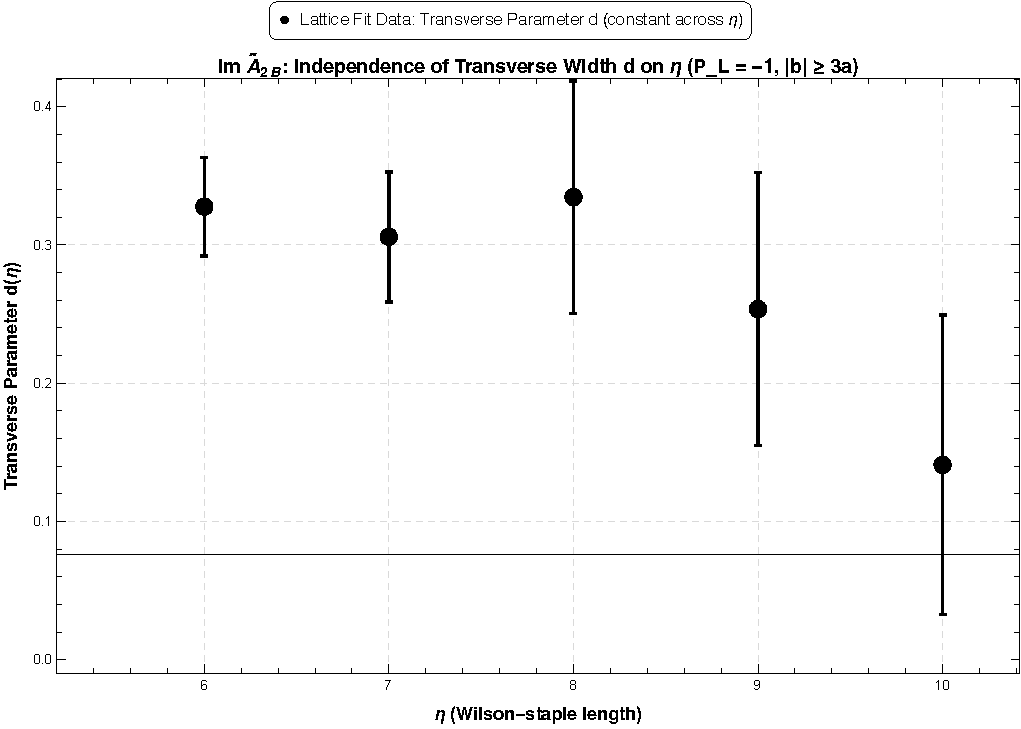
\includegraphics[width=0.49\linewidth]{PowerLaw_etaAsymptotic/ImA2B_d_eta_Independence_P1.pdf}
    \caption{Lattice extracted parameters $c$ (left) and $d$ (right) for $\tAmp_{2B}^{\text{Im}}$ as a function of $\eta$. Despite increased statistical noise, the data are highly consistent with the constant-parameter ansatz.}
    \label{fig:ImA2B_eta_independence}
\end{figure}

The analytical models in invariant $(b_L,b_T)$ space for the three amplitudes are:
\begin{align}
    \tAmp_{2B}^{\text{Re}}&=\left[\frac{a e^{-f \eta}}{\left[1 + \left(d + c\left(1 - \frac{k_1}{\eta} - \frac{k_2}{\eta^2}\right)\right) b_L^2 + d b_T^2\right]^j}\right]\label{eq:model_ReA2B}\\
    \tAmp_{12B}^{\text{Re}}&=\left[\frac{-a^{\prime} e^{-f \eta}}{\left[1 + (c^{\prime} + d^{\prime}) b_L^2 + d^{\prime} b_T^2\right]^{j^{\prime}}}\right]\label{eq:model_ReA12B}\\
    \tAmp_{2B}^{\text{Im}}&=\left[\frac{a^{\prime\prime} b_L e^{-f \eta}}{\left[1 + (c^{\prime\prime} + d^{\prime\prime}) b_L^2 + d^{\prime\prime} b_T^2\right]^{j^{\prime\prime}}}\right]\label{eq:model_ImA2B}
\end{align}


\subsection{Simultaneous Fitting Strategy}
\label{sec:simultaneous_fit_strategy}

The structural models in Eq. (\ref{eq:model_ReA2B})-(\ref{eq:model_ImA2B}) show that all three surviving amplitudes share an $\eta$-dependence damped by a common exponential decay factor, $e^{-f\eta}$. Because the Sivers shift is a ratio of transverse momentum moments, this shared exponential behavior cancels out in the physical momentum fraction $x$ calculation. 

The Sivers shift is the ratio of the first transverse momentum moment of the Sivers function to the unpolarized TMD distribution:
\begin{equation}
   \langle \vect{k}_y \rangle_{TU}(\vprp{\bvec}^2,x,\zetahat,\eta v \tcdot P) 
	\ \equiv\ \mN \frac{\tilde f_{1T}^{\perp(1)}(\vprp{\bvec}^2;\zetahat,\ldots,\eta v \tcdot P)}{\tilde f_1^{(0)}(\vprp{\bvec}^2;\zetahat,\ldots,\eta v \tcdot P)} \ .
\end{equation}

Expanding these Fourier-transformed distributions in terms of the invariant effective amplitudes $\tAmp_{12B}$ and $\tAmp_{2B}$, we rewrite the ratio as an integration over the longitudinal quark spatial separation $b \cdot P$:
\begin{equation}
    \langle \vect{k}_y \rangle_{TU} = -m_{N} \frac{\int d(b\cdot P)e^{ix(b\cdot P)} \tAmp_{12B}(\bvec^2,\bvec \tcdot P,(\bvec \tcdot P) R(\zetahat^2)/\mN^2,-1/(\mN\zetahat)^2,\eta v \tcdot P)}{\int d(b\cdot P)e^{ix(b\cdot P)}\tAmp_{2B}(\bvec^2,\bvec \tcdot P,(\bvec \tcdot P) R(\zetahat^2)/\mN^2,-1/(\mN\zetahat)^2,\eta v \tcdot P)} \ .
\end{equation}

We then decompose the complex effective amplitudes into their real (T-even) and imaginary (T-odd) components. The imaginary Sivers amplitude is statistically consistent with zero, so we remove $\tAmp_{12B}^{\text{Im}}$ from the numerator:
\begin{equation}
    \langle \vect{k}_y \rangle_{TU} = -m_{N} \frac{\int d(b\cdot P)e^{ix(b\cdot P)} \left[\tAmp_{12B}^{\text{Re}}(\cdots)+i\cancelto{0}{\tAmp_{12B}^{\text{Im}}(\cdots)}\right]}{\int d(b\cdot P)e^{ix(b\cdot P)}\left[\tAmp_{2B}^{\text{Re}}(\cdots)+i\tAmp_{2B}^{\text{Im}}(\cdots)\right]} \ .
\end{equation}

We use Euler's formula to expand the Fourier kernel $e^{ix(b\cdot P)}$ into cosine and sine components. Because the integration domain is symmetric, any integrand that is odd in $b \cdot P$ integrates to zero. Retaining only the non-vanishing even-parity combinations yields:
\begin{equation}
    \langle \vect{k}_y \rangle_{TU} = -m_{N} \frac{\int d(b\cdot P) \cos{\left(x(b\cdot P)\right)}\tAmp_{12B}^{\text{Re}}(\cdots)}{\int d(b\cdot P)\left[\cos{\left(x(b\cdot P)\right)}\tAmp_{2B}^{\text{Re}}(\cdots)-\sin{\left(x(b\cdot P)\right)}\tAmp_{2B}^{\text{Im}}(\cdots)\right]} \ .
\end{equation}
Substituting the analytical models from Eq. (\ref{eq:model_ReA2B})-(\ref{eq:model_ImA2B}) shows the shared asymptotic parameter $e^{-f \eta}$. Because the $e^{-f\eta}$ term is independent of the integration variable $b \cdot P$, it factors out of both the numerator and denominator integrals, canceling the shared exponential decay parameter. Applying the Lorentz-invariant projection $b_L = \frac{P \cdot b}{-P_L}$ and $b_T^2=b^2-b_L^2$, we arrive at the final integrands in the invariant frame:
\begin{equation}
\begin{aligned}
    \langle \vect{k}_y \rangle_{TU} &= m_{N} \frac{\int d(b\cdot P) \cos{\left(x(b\cdot P)\right)} \frac{a^{\prime}}{D_{12B}^{\text{Re}}}}{\int d(b\cdot P)\left[\cos{\left(x(b\cdot P)\right)} \frac{a}{D_{2B}^{\text{Re}}} - \sin{\left(x(b\cdot P)\right)}\frac{a^{\prime\prime} (P \cdot b) / (-P_L)}{D_{2B}^{\text{Im}}}\right]} \ , \\
    D_{12B}^{\text{Re}} &= \left[1 + (c^{\prime}) \frac{(P \cdot b)^2}{P_L^2} + d^{\prime} b^2\right]^{j^{\prime}} \ , \\
    D_{2B}^{\text{Re}} &= \left[1 + \left(c\left(1 - \frac{k_1}{\eta} - \frac{k_2}{\eta^2}\right)\right) \frac{(P \cdot b)^2}{P_L^2} + d b^2\right]^j \ , \\
    D_{2B}^{\text{Im}} &= \left[1 + (c^{\prime\prime}) \frac{(P \cdot b)^2}{P_L^2} + d^{\prime\prime} b^2\right]^{j^{\prime\prime}} \ .
\end{aligned}
\end{equation}
To enforce this shared $\eta$-dependence across the amplitudes, we use a simultaneous global fit. Forcing the parameter $f$ to be identical across all three amplitude models ($\tAmp_{2B}^{\text{Re}}$, $\tAmp_{2B}^{\text{Im}}$, and $\tAmp_{12B}^{\text{Re}}$) ensures theoretical consistency and stabilizes the parameter extraction, reflecting the physical cancellation mechanism above.


For the unpolarized real amplitude $\tAmp_{2B}^{\text{Re}}$, the transverse width parameter $d$ remains constant across all $\eta$, but the longitudinal width parameter $c(\eta)$ requires an asymptotic model.

In selecting the final model for $c(\eta)$, statistical goodness-of-fit must be paired with physical boundary conditions on the light-cone momentum fraction $x \in [-1, 1]$:

\begin{itemize}
    \item \textbf{Quark versus Anti-quark Domains}: In light-cone field theory, positive momentum fractions ($x > 0$) correspond to quark distributions $q(x) = f_1(x)$, while negative momentum fractions ($x < 0$) govern anti-quark distributions through $\bar{q}(x) = -f_1(-x)$.
    \item \textbf{Anti-quark Suppression at Large $|x|$}: In physical nucleons, sea anti-quark densities are concentrated strictly at low momentum fractions ($|x| \lesssim 0.1$). As $|x|$ increases, the anti-quark distribution falls rapidly to zero. At moderate-to-large values ($x < -0.2$ or $x < -0.3$), the anti-quark density is negligible.
    \item \textbf{Fourier Artifact Suppression}: Candidate models that approach the asymptote too slowly or fail to capture the curvature in $\eta$ (such as Candidates 2 and 5) produce unphysical oscillatory behavior or non-vanishing tails in the negative-$x$ region ($x < -0.2$) upon Fourier transformation. Candidate 1 cleanly suppresses anti-quark contributions in this regime while maintaining an optimal balance of minimal $\chi^2/\text{dof}$ and AIC score.
\end{itemize}

\subsubsection{Simultaneous Fit with Full Covariance Matrix}

Because we extract the amplitudes from the same gauge field configurations and evaluate them across nearby spatial coordinates $(b_L, b_T)$, their statistical fluctuations are highly correlated. A simple uncorrelated $\chi^2$ minimization improperly weights these data points, deflating uncertainties and biasing the central values.

To resolve this, we perform a correlated $\chi^2$ minimization utilizing the full covariance matrix. This accounts for the cross-correlations inherent in the lattice data, both across different quark spatial separations and across the real and imaginary amplitude components. 

We estimate these correlations using Jackknife resampling. Let $y_i^{(k)}$ represent the lattice evaluation of the $i$-th data point (spanning all spatial coordinates across $\tAmp_{2B}^{\text{Re}}$, $\tAmp_{2B}^{\text{Im}}$, and $\tAmp_{12B}^{\text{Re}}$) in the $k$-th Jackknife bin. The full Jackknife covariance matrix $C_{ij}$ is defined as \cite{Boram2011Covariance}:
\begin{equation}
    C_{ij} = \frac{N-1}{N} \sum_{k=1}^{N} \left( y_i^{(k)} - \bar{y}_i \right) \left( y_j^{(k)} - \bar{y}_j \right) \ ,
\end{equation}
where $N$ is the total number of Jackknife samples and $\bar{y}_i = \frac{1}{N}\sum_k y_i^{(k)}$ is the sample mean. 

The global simultaneous fit minimizes the correlated $\chi^2$ objective function with respect to the model parameters $\mathbf{p}$:
\begin{equation}
    \chi^2(\mathbf{p}) = \sum_{i,j} \left( \bar{y}_i - F_i(\mathbf{p}) \right) C_{ij}^{-1} \left( \bar{y}_j - F_j(\mathbf{p}) \right) \ ,
\end{equation}
where $F_i(\mathbf{p})$ represents the analytical models evaluated at the corresponding kinematics. 

We utilize the \texttt{lsqfit} \cite{Lepage:2001ym} non-linear least squares fitting package and the \texttt{gvar} library for Gaussian error propagation. We construct the full Jackknife covariance matrix that captures the cross-correlations between $\tAmp_{2B}^{\text{Re}}$, $\tAmp_{2B}^{\text{Im}}$, and $\tAmp_{12B}^{\text{Re}}$. The \texttt{gvar} framework binds the combined lattice data array to the inverse covariance matrix.

\subsection{Rejection of Separable Longitudinal and Transverse Factorization}
\label{sec:rejection_exponential_longitudinal}
To test this separability hypothesis discussed in Section \ref{Test-for-Factorization}, we constructed candidate models that multiply an independent longitudinal profile by various transverse $b^2$ profiles, including combinations of Gaussian, Lorentzian power-law, and exponential-decay forms. We evaluated each model with full Jackknife fits.

The fit results are summarized in Fig.~\ref{fig:rejection_exponential_longitudinal}. When exponential decay in $(P\cdot b)$ is paired with a Gaussian transverse profile, the fit is poor ($\chi^2/\text{dof} \approx 4.98$). Even for the other models, the $\chi^2/\text{dof} \approx 2$, and the coefficient $c$ governing the $(P\cdot b)$ evaluates to a negative value and is also consistent with zero within Jackknife uncertainties; this is unstable and divergent when performing a Fourier transform. 

\begin{figure}[htbp]
    \centering
    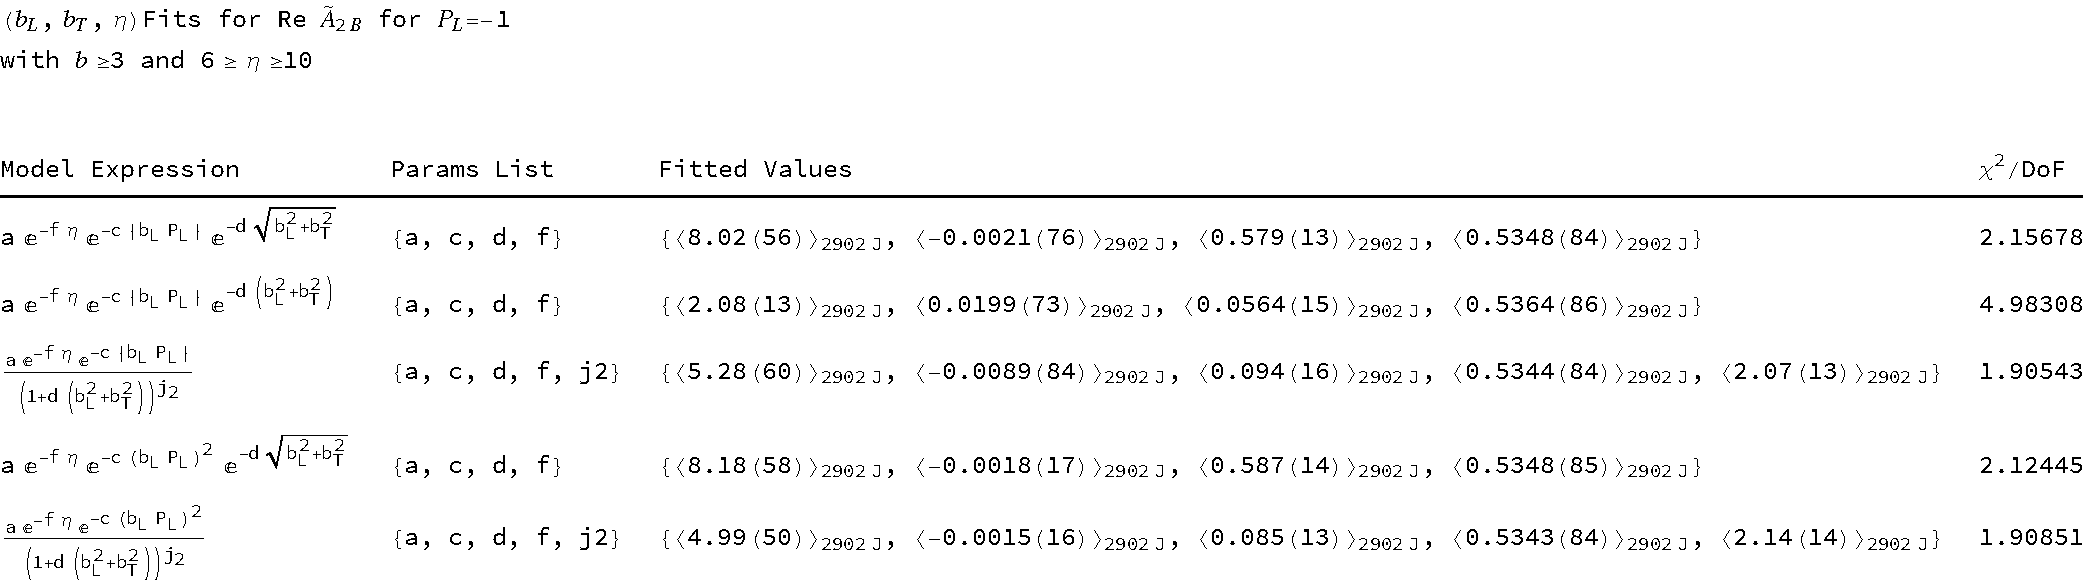
\includegraphics[width=1\linewidth]{plots/Rejection-of-Separable-Exponential-Longitudinal-Decay.pdf}
    \caption{Fit results testing the validity of the separability hypothesis: an exponential decay in $(P\cdot b)$ is paired with a Gaussian transverse profile; the fit is poor ($\chi^2/\text{dof} \approx 4.98$). In models that achieve a lower $\chi^2/\text{dof}$, the coefficient $c$ consistently fits to zero within uncertainties and is negative in each Jackknife set, demonstrating that the data rejects the separability hypothesis.}
    \label{fig:rejection_exponential_longitudinal}
\end{figure}

We also explored the separability hypothesis with $\eta$-dependent $c$, as $c(\eta)$, which governs $(P\cdot b)$; in the asymptotic limit, this forces $c$ to be positive. By introducing the asymptotic $c(\eta)$, we lowered the $\chi^2/\text{dof}$ to $ \approx 1.35$, and in the asymptotic limit $c$ is positive. From the fitting routine, we find that the lattice data prefer a power-law in $(P \cdot b)$ rather than an exponential decay in $|(P \cdot b)|$.
\begin{figure}[htbp]
    \centering
    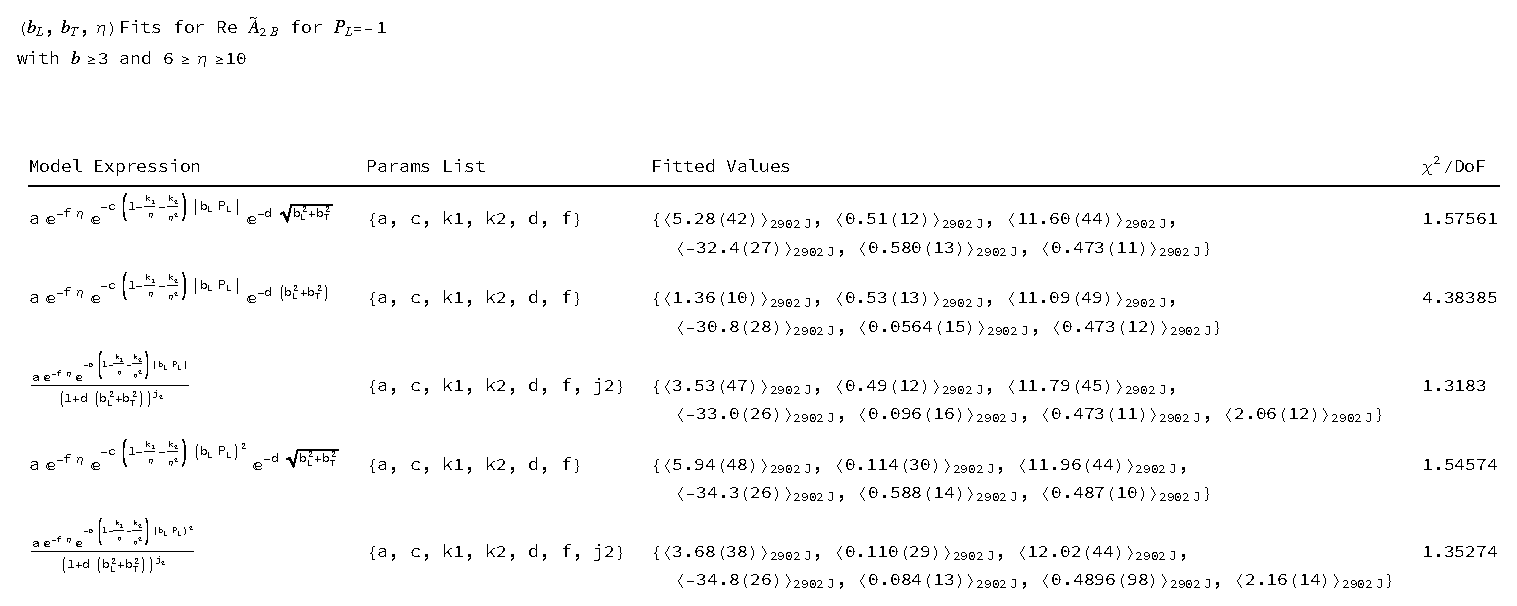
\includegraphics[width=1\linewidth]{plots/Rejection-of-Separable-Exponential-Longitudinal-Decay-ceta.eps}
    \caption{Fit results testing the validity of the separability hypothesis with $\eta$-dependent $c$, as $c(\eta)$. In models that achieve a lower $\chi^2/\text{dof}$, the coefficient $c$ is now positive}
    \label{fig:rejection_exponential_longitudinal}
\end{figure}


We systematically investigated four distinct factorized ansatze with lower $\chi^2/\text{dof}$ and propagated the same ansatze to all three invariant amplitudes ($\tAmp_{2B}^{\text{Re}}$, $\tAmp_{2B}^{\text{Im}}$, and $\tAmp_{12B}^{\text{Re}}$). These models combine either an exponential ($e^{-c|P\cdot b|}$) or Gaussian ($e^{-c(P\cdot b)^2}$) longitudinal profile with either an exponential ($e^{-d|b|}$) or power-law ($(1+db^2)^{-j}$) transverse envelope:
\begin{enumerate}
    \item \textbf{\texttt{ExpPb\_Expb}}:
    \begin{align}
        \tAmp_{2B}^{\text{Re}} &= a_{\text{re}} \, e^{-c_{\text{re}}|P\cdot b| - d_{\text{re}}|b|} \, e^{-f\eta} \ , \\
        \tAmp_{2B}^{\text{Im}} &= a_{\text{im}} \, (P\cdot b) \, e^{-c_{\text{im}}|P\cdot b| - d_{\text{im}}|b|} \, e^{-f\eta} \ , \\
        \tAmp_{12B}^{\text{Re}} &= -a_{\text{reA12B}} \, e^{-c_{\text{reA12B}}|P\cdot b| - d_{\text{reA12B}}|b|} \, e^{-f\eta} \ .
    \end{align}
    
    \item \textbf{\texttt{ExpPb\_PowerLawb}}:
    \begin{align}
        \tAmp_{2B}^{\text{Re}} &= \frac{a_{\text{re}} \, e^{-c_{\text{re}}|P\cdot b| - f\eta}}{\left(1 + d_{\text{re}} b^2\right)^{j_{\text{re}}}} \ , \\
        \tAmp_{2B}^{\text{Im}} &= \frac{a_{\text{im}} \, (P\cdot b) \, e^{-c_{\text{im}}|P\cdot b| - f\eta}}{\left(1 + d_{\text{im}} b^2\right)^{j_{\text{im}}}} \ , \\
        \tAmp_{12B}^{\text{Re}} &= \frac{-a_{\text{reA12B}} \, e^{-c_{\text{reA12B}}|P\cdot b| - f\eta}}{\left(1 + d_{\text{reA12B}} b^2\right)^{j_{\text{reA12B}}}} \ .
    \end{align}

    \item \textbf{\texttt{GaussianPb\_Expb}}:
    \begin{align}
        \tAmp_{2B}^{\text{Re}} &= a_{\text{re}} \, e^{-c_{\text{re}}(P\cdot b)^2 - d_{\text{re}}|b|} \, e^{-f\eta} \ , \\
        \tAmp_{2B}^{\text{Im}} &= a_{\text{im}} \, (P\cdot b) \, e^{-c_{\text{im}}(P\cdot b)^2 - d_{\text{im}}|b|} \, e^{-f\eta} \ , \\
        \tAmp_{12B}^{\text{Re}} &= -a_{\text{reA12B}} \, e^{-c_{\text{reA12B}}(P\cdot b)^2 - d_{\text{reA12B}}|b|} \, e^{-f\eta} \ .
    \end{align}

    \item \textbf{\texttt{GaussianPb\_PowerLawb}}:
    \begin{align}
        \tAmp_{2B}^{\text{Re}} &= \frac{a_{\text{re}} \, e^{-c_{\text{re}}(P\cdot b)^2 - f\eta}}{\left(1 + d_{\text{re}} b^2\right)^{j_{\text{re}}}} \ , \\
        \tAmp_{2B}^{\text{Im}} &= \frac{a_{\text{im}} \, (P\cdot b) \, e^{-c_{\text{im}}(P\cdot b)^2 - f\eta}}{\left(1 + d_{\text{im}} b^2\right)^{j_{\text{im}}}} \ , \\
        \tAmp_{12B}^{\text{Re}} &= \frac{-a_{\text{reA12B}} \, e^{-c_{\text{reA12B}}(P\cdot b)^2 - f\eta}}{\left(1 + d_{\text{reA12B}} b^2\right)^{j_{\text{reA12B}}}} \ .
    \end{align}
\end{enumerate}

Each model admits closed-form analytical Fourier transforms, which makes it straightforward to inspect the resulting $x$-space distributions. We performed global simultaneous Jackknife fits on these four ansatze using the same kinematic cuts ($|\vect{b}| \ge 3a$, $\eta \in [6, 10]$) and shared area-law factor $e^{-f\eta}$. The fit quality and extracted parameters are summarized in Table~\ref{tab:factorized_ansatze_comparison}.

\begin{table}[htbp]
\centering
\renewcommand{\arraystretch}{1.3}
\caption{Comparison of the four factorized longitudinal-transverse models across nucleon momenta $P_L$, with extracted parameters shown at $P_L = -1$. While models with power-law transverse envelopes describe $\tAmp_{2B}^{\text{Re}}$ passably, all four factorized ansatze fail on $\tAmp_{2B}^{\text{Im}}$ and $\tAmp_{12B}^{\text{Re}}$.}
\label{tab:factorized_ansatze_comparison}
\scalebox{0.7}{
\begin{tabular}{|l|c|c|c|c|c|c|c|p{4.2cm}|}
\hline
\textbf{Model Ansatz} & \multicolumn{4}{c|}{\textbf{$\chi^2/\text{dof}$ Across Momenta}} & \multicolumn{3}{c|}{\textbf{Key Fitted Parameters at $P_L = -1$}} & \textbf{Primary Failure Mode} \\
\cline{2-8}
& $P_L = -1$ & $P_L = -2$ & $P_L = -3$ & $P_L = -4$ & $c_{\text{im}}$ & $c_{\text{reA12B}}$ & $a_{\text{im}}$ & \\
\hline
\texttt{ExpPb\_Expb} & $1.406(92)$ & $0.956(75)$ & $0.622(61)$ & $0.455(53)$ & $0.0010(262)$ & $0.045(23)$ & $-0.167(16)$ & $c_{\text{im}} \to 0$; unphysical sign on $a_{\text{im}}$. \\
\hline
\texttt{ExpPb\_PowerLawb} & $1.286(89)$ & $0.938(75)$ & $0.623(61)$ & $0.447(53)$ & $0.0045(248)$ & $0.028(24)$ & $-0.167(31)$ & Fits $\tAmp_{2B}^{\text{Re}}$ well, but $c_{\text{im}}$ and $c_{\text{reA12B}}$ vanish within error; flips sign of $a_{\text{im}}$. \\
\hline
\texttt{GaussianPb\_Expb} & $2.389(121)$ & $2.005(111)$ & $0.945(76)$ & $0.453(52)$ & $0.568(171)$ & $0.0038(69)$ & $+0.050(121)$ & Poor $\chi^2/\text{dof}$; $c_{\text{reA12B}}$ pinned near zero; Gaussian over-damping at large $x$. \\
\hline
\texttt{GaussianPb\_PowerLawb} & $2.316(120)$ & $1.981(111)$ & $0.948(76)$ & $0.448(52)$ & $0.602(48)$ & $0.0016(61)$ & $+0.168(92)$ & Poor global fit at low momenta; $c_{\text{reA12B}} \approx 0$; unphysical truncation of valence tails. \\
\hline
\textbf{Coupled Lorentzian} & \multicolumn{4}{c|}{\textbf{$1.85(10)$ (Correlated Covariance Fit)}} & $\mathbf{0.2253(69)}$ & $\mathbf{0.0773(46)}$ & $\mathbf{+0.267(13)}$ & \textbf{All parameters stable, positive, and well-constrained across all amplitudes.} \\
\hline
\end{tabular}
}
\end{table}

The numerical results highlight several critical failure mechanisms inherent to factorized models. In \texttt{ExpPb\_PowerLawb}, the real unpolarized amplitude fits with $\chi^2/\text{dof} \approx 1.286$. Because $\tAmp_{2B}^{\text{Re}}$ dominates the statistical weight, an uncritical fit can give the false impression of an adequate model. However, the same parameterization fails for the imaginary amplitude $\tAmp_{2B}^{\text{Im}}$: the longitudinal decay width $c_{\text{im}} = 0.0045 \pm 0.0248$ evaluates to zero within errors. This means the model loses its longitudinal decay profile, producing an essentially flat distribution in $P\cdot b$. Furthermore, the overall amplitude flips to an unphysical negative sign ($a_{\text{im}} = -0.167$).

For the real Sivers amplitude $\tAmp_{12B}^{\text{Re}}$, the longitudinal parameter $c_{\text{reA12B}}$ is similarly suppressed across all factorized models ($0.028 \pm 0.024$ for \texttt{ExpPb\_PowerLawb} and $0.0016 \pm 0.0061$ for \texttt{GaussianPb\_PowerLawb}). The factorized models cannot capture the distinct longitudinal curvature of the spin-dependent correlator without forcing the decay parameter to its lower boundary. Factoring out an exponential $|P\cdot b|$ dependence introduces a discontinuous first derivative (a cusp) at $P\cdot b = 0$. For an odd-parity amplitude like $\tAmp_{2B}^{\text{Im}}$, which must vanish linearly through the origin ($\tAmp_{2B}^{\text{Im}} \propto b_L$), the non-analytic factor $e^{-c|P\cdot b|}$ conflicts with the smooth behavior of the Euclidean correlation function. The fit responds by driving $c_{\text{im}} \to 0$ to minimize the cusp penalty.

In the Lorentz-invariant variable space $(P\cdot b, b^2)$, the longitudinal separation $b_L = (P\cdot b)/(-P_L)$ and transverse separation $b_T = \sqrt{b^2 - b_L^2}$ are geometrically coupled. Factorized models force an artificial independence between $P\cdot b$ and $b^2$. In contrast, coupling $(P\cdot b)^2$ and $b^2$ within a single denominator,
    \begin{equation}
        D = \left[ 1 + c(\eta) \frac{(P\cdot b)^2}{P_L^2} + d\,b^2 \right]^j \ ,
    \end{equation}
preserves smooth analyticity at $P\cdot b = 0$, satisfies power-law integrability, and yields stable, positive parameters across all three amplitudes (e.g., $c_{\text{im}} = 0.2253(69)$, $c_{\text{reA12B}} = 0.0773(46)$, $a_{\text{im}} = +0.267(13)$). We therefore exclude factorized ansatze and adopt the coupled Lorentzian denominator for the global analysis.

The following subsections present the results of these simultaneous covariance matrix fits evaluated at discrete lattice momenta.

\renewcommand{\PLval}{-1}
\subsubsection{\texorpdfstring{Simultaneous Fit Results for $\vect{P}\cdot a\hat{L}/(2\pi)=\{\PLval,0,0\}$}{TEXT}}

The extracted parameters from the simultaneous fit for the lowest simulated nucleon momentum, $P_1 = -1$ ($\hat{\zeta} \approx 0.091$), are summarized below. Enforcing the shared asymptotic decay parameter $f$ across all three effective amplitudes ($\tAmp_{2B}^{\text{Re}}$, $\tAmp_{2B}^{\text{Im}}$, and $\tAmp_{12B}^{\text{Re}}$) stabilizes the extraction of the spatial profiles and preserves the cancellation required for the Sivers shift ratio.

\input{SimultaneousFitsCov/Fit_Table_PL\PLval_bmin3}

Figures \ref{fig:A2B_amplitudes_fit_P1} and \ref{fig:combined_fit_P1} show the results of the correlated minimization. The parameterization, shown as continuous surfaces with shaded error bands, matches the discrete lattice data across the Cartesian $(b_L/a, b_T/a)$ grid and the Lorentz-invariant $(P \cdot b, b^2)$ variable space. Excluding the short-distance data ($|\vect{b}| < 3a$) ensures the fit captures long-range dynamics without ultraviolet lattice artifacts skewing the results.

\begin{figure}[htbp]
    \centering
    \begin{tabular}{ccc}
        % Column Headers
        \textbf{$\widetilde{A}^{Re}_{2B}$} & \textbf{$\widetilde{A}^{Im}_{2B}$} & \textbf{$\widetilde{A}^{Re}_{12B}$} \\[2ex]
        \includegraphics[width=0.3\linewidth]{plots/Amps_Fit/ReA12B_Pb_bsq_PL\PLval_WithFit_3D.pdf} &
        \includegraphics[width=0.3\linewidth]{plots/Amps_Fit/ImA2B_PL\PLval_WithFit_3D.pdf} &
        \includegraphics[width=0.3\linewidth]{plots/Amps_Fit/ReA12B_PL\PLval_WithFit_3D.pdf}\\[2ex]
        \includegraphics[width=0.3\linewidth]{plots/Amps_Fit/ReA2B_Pb_bsq_PL\PLval_WithFit_3D.pdf} &
        \includegraphics[width=0.3\linewidth]{plots/Amps_Fit/ImA2B_Pb_bsq_PL\PLval_WithFit_3D.pdf} &
        \includegraphics[width=0.3\linewidth]{plots/Amps_Fit/ReA12B_Pb_bsq_PL\PLval_WithFit_3D.pdf} \\
    \end{tabular}
    \caption{Fit for $\widetilde{A}^{Re}_{2B}$, $\widetilde{A}^{Im}_{2B}$ \& $\widetilde{A}^{Re}_{12B}$ amplitudes for $\vect{P}\cdot a\hat{L}/(2\pi)=\{\PLval,0,0\}$. The top row displays the $(b_{L}/a,b_{T}/a,\eta|\vect{v}|/a)-$space, while the bottom row displays the $((\vect{P}\cdot \vect{b})\cdot\hat{L}/(2\pi),b^{2}/a^2,\eta|\vect{v}|/a)-$space with the global simultaneous fit overlaid.}
    \label{fig:A2B_amplitudes_fit_P1}
\end{figure}

\begin{figure}[htbp]
    \centering
    \begin{tabular}{c}
        \includegraphics[width=0.9\linewidth]{plots/Amps_Fit/Combined_eta8_PL\PLval_WithFit_2D.pdf} \\
        \includegraphics[width=0.9\linewidth]{plots/Amps_Fit/Combined_Pb_bsq_eta8_PL\PLval_WithFit_2D.pdf} \\
    \end{tabular}
    \caption{Fit for $\widetilde{A}^{Re}_{2B}$, $\widetilde{A}^{Im}_{2B}$ \& $\widetilde{A}^{Re}_{12B}$ amplitudes for $\vect{P}\cdot a\hat{L}/(2\pi)=\{\PLval,0,0\}$ at a fixed staple extent $\eta|\vect{v}|/a=8$. The top two rows display the $(b_{L}/a,b_{T}/a)-$space, while the bottom two rows display the $((\vect{P}\cdot \vect{b})\cdot\hat{L}/(2\pi),b^{2}/a^2)-$space with the fit.}
    \label{fig:combined_fit_P1}
\end{figure}

\pagebreak

Using the continuous parametrization of the effective amplitudes, we analytically evaluate the Fourier integrals over the invariant scalar $P \cdot b$. The results of these integrations, which yield the momentum fraction $x$-dependent unpolarized distribution and the Sivers shift, are tabulated below.

\input{SimultaneousFitsCov/Integration_Table_PL\PLval_bmin3}

The figures below show the Jackknife covariance matrix. The off-diagonal elements in the 2D correlation matrix and the 3D surface plot show cross-correlations between spatial lattice points and across amplitude components. Incorporating this covariance structure into the fitting pipeline via \texttt{lsqfit} properly weights the correlated fluctuations to determine the error bands on the final extracted Sivers shift.

\begin{figure}[htbp]
    \centering
    \includegraphics[width=0.5\linewidth]{SimultaneousFitsCov/SimulFitCovMatrix-A12B-A2B-FT-a_im-a_re-a_reA12B-c_im-c_re-c_reA12B-d_im-d_re-d_reA12B-f-j_im-j_re-j_reA12B-k1_re-k2_re__bmin3_eta610_PL\PLval.pdf}
    \caption{2D representation of the full Jackknife covariance matrix utilized in the simultaneous fit for $P_1=-1$. The prominent off-diagonal bands highlight the strong correlations across the parameter space.}
    \label{fig:cov_matrix_2d_P1}
\end{figure}

\begin{figure}[htbp]
    \centering
    \includegraphics[width=0.7\linewidth]{SimultaneousFitsCov/SimulFitCovMatrix-A12B-A2B-FT-3D_a_im-a_re-a_reA12B-c_im-c_re-c_reA12B-d_im-d_re-d_reA12B-f-j_im-j_re-j_reA12B-k1_re-k2_re__bmin3_eta610_PL\PLval.pdf}
    \caption{3D surface plot of the Jackknife covariance matrix for $P_1=-1$, visually emphasizing the magnitude of the cross-correlations between the real and imaginary amplitude components.}
    \label{fig:cov_matrix_3d_P1}
\end{figure}
\pagebreak

\pagebreak
\renewcommand{\PLval}{-2}
\subsubsection{\texorpdfstring{Simultaneous Fit Results for $\vect{P}\cdot a\hat{L}/(2\pi)=\{\PLval,0,0\}$}{TEXT}}
\input{SimultaneousFitsCov/Fit_Table_PL\PLval_bmin3}
\begin{figure}[htbp]
    \centering
    \begin{tabular}{ccc}
        % Column Headers
        \textbf{$\widetilde{A}^{Re}_{2B}$} & \textbf{$\widetilde{A}^{Im}_{2B}$} & \textbf{$\widetilde{A}^{Re}_{12B}$} \\[2ex]
        \includegraphics[width=0.3\linewidth]{plots/Amps_Fit/ReA12B_Pb_bsq_PL\PLval_WithFit_3D.pdf} &
        \includegraphics[width=0.3\linewidth]{plots/Amps_Fit/ImA2B_PL\PLval_WithFit_3D.pdf} &
        \includegraphics[width=0.3\linewidth]{plots/Amps_Fit/ReA12B_PL\PLval_WithFit_3D.pdf}\\[2ex]
        \includegraphics[width=0.3\linewidth]{plots/Amps_Fit/ReA2B_Pb_bsq_PL\PLval_WithFit_3D.pdf} &
        \includegraphics[width=0.3\linewidth]{plots/Amps_Fit/ImA2B_Pb_bsq_PL\PLval_WithFit_3D.pdf} &
        \includegraphics[width=0.3\linewidth]{plots/Amps_Fit/ReA12B_Pb_bsq_PL\PLval_WithFit_3D.pdf} \\
    \end{tabular}
    \caption{Fit for $\widetilde{A}^{Re}_{2B}$, $\widetilde{A}^{Im}_{2B}$ \& $\widetilde{A}^{Re}_{12B}$ amplitudes for $\vect{P}\cdot a\hat{L}/(2\pi)=\{\PLval,0,0\}$. The top row displays the $(b_{L}/a,b_{T}/a,\eta|\vect{v}|/a)-$space, while the bottom row displays the $((\vect{P}\cdot \vect{b})\cdot\hat{L}/(2\pi),b^{2}/a^2,\eta|\vect{v}|/a)-$space with the global simultaneous fit overlaid.}
    \label{fig:A2B_amplitudes_fit_P2}
\end{figure}

\begin{figure}[htbp]
    \centering
    \begin{tabular}{c}
        \includegraphics[width=0.9\linewidth]{plots/Amps_Fit/Combined_eta8_PL\PLval_WithFit_2D.pdf} \\
        \includegraphics[width=0.9\linewidth]{plots/Amps_Fit/Combined_Pb_bsq_eta8_PL\PLval_WithFit_2D.pdf} \\
    \end{tabular}
    \caption{Fit for $\widetilde{A}^{Re}_{2B}$, $\widetilde{A}^{Im}_{2B}$ \& $\widetilde{A}^{Re}_{12B}$ amplitudes for $\vect{P}\cdot a\hat{L}/(2\pi)=\{\PLval,0,0\}$ at a fixed staple extent $\eta|\vect{v}|/a=8$. The top two rows display the $(b_{L}/a,b_{T}/a)-$space, while the bottom two rows display the $((\vect{P}\cdot \vect{b})\cdot\hat{L}/(2\pi),b^{2}/a^2)-$space with the fit.}
    \label{fig:combined_fit_P2}
\end{figure}

\pagebreak
\input{SimultaneousFitsCov/Integration_Table_PL\PLval_bmin3}

\begin{figure}[htbp]
    \centering
    \includegraphics[width=0.5\linewidth]{SimultaneousFitsCov/SimulFitCovMatrix-A12B-A2B-FT-a_im-a_re-a_reA12B-c_im-c_re-c_reA12B-d_im-d_re-d_reA12B-f-j_im-j_re-j_reA12B-k1_re-k2_re__bmin3_eta610_PL\PLval.pdf}
    \caption{2D representation of the full Jackknife covariance matrix utilized in the simultaneous fit for $P_L=-2$.}
    \label{fig:cov_matrix_2d_P2}
\end{figure}

\begin{figure}[htbp]
    \centering
    \includegraphics[width=0.7\linewidth]{SimultaneousFitsCov/SimulFitCovMatrix-A12B-A2B-FT-3D_a_im-a_re-a_reA12B-c_im-c_re-c_reA12B-d_im-d_re-d_reA12B-f-j_im-j_re-j_reA12B-k1_re-k2_re__bmin3_eta610_PL\PLval.pdf}
    \caption{3D surface plot of the Jackknife covariance matrix for $P_L=-2$.}
    \label{fig:cov_matrix_3d_P2}
\end{figure}

\pagebreak
\renewcommand{\PLval}{-3}
\subsubsection{\texorpdfstring{Simultaneous Fit Results for $\vect{P}\cdot a\hat{L}/(2\pi)=\{\PLval,0,0\}$}{TEXT}}
\input{SimultaneousFitsCov/Fit_Table_PL\PLval_bmin3}
\begin{figure}[htbp]
    \centering
    \begin{tabular}{ccc}
        % Column Headers
        \textbf{$\widetilde{A}^{Re}_{2B}$} & \textbf{$\widetilde{A}^{Im}_{2B}$} & \textbf{$\widetilde{A}^{Re}_{12B}$} \\[2ex]
        \includegraphics[width=0.3\linewidth]{plots/Amps_Fit/ReA12B_Pb_bsq_PL\PLval_WithFit_3D.pdf} &
        \includegraphics[width=0.3\linewidth]{plots/Amps_Fit/ImA2B_PL\PLval_WithFit_3D.pdf} &
        \includegraphics[width=0.3\linewidth]{plots/Amps_Fit/ReA12B_PL\PLval_WithFit_3D.pdf}\\[2ex]
        \includegraphics[width=0.3\linewidth]{plots/Amps_Fit/ReA2B_Pb_bsq_PL\PLval_WithFit_3D.pdf} &
        \includegraphics[width=0.3\linewidth]{plots/Amps_Fit/ImA2B_Pb_bsq_PL\PLval_WithFit_3D.pdf} &
        \includegraphics[width=0.3\linewidth]{plots/Amps_Fit/ReA12B_Pb_bsq_PL\PLval_WithFit_3D.pdf} \\
    \end{tabular}
    \caption{Fit for $\widetilde{A}^{Re}_{2B}$, $\widetilde{A}^{Im}_{2B}$ \& $\widetilde{A}^{Re}_{12B}$ amplitudes for $\vect{P}\cdot a\hat{L}/(2\pi)=\{\PLval,0,0\}$. The top row displays the $(b_{L}/a,b_{T}/a,\eta|\vect{v}|/a)-$space, while the bottom row displays the $((\vect{P}\cdot \vect{b})\cdot\hat{L}/(2\pi),b^{2}/a^2,\eta|\vect{v}|/a)-$space with the global simultaneous fit overlaid.}
    \label{fig:A2B_amplitudes_fit_P3}
\end{figure}

\begin{figure}[htbp]
    \centering
    \begin{tabular}{c}
        \includegraphics[width=0.9\linewidth]{plots/Amps_Fit/Combined_eta8_PL\PLval_WithFit_2D.pdf} \\
        \includegraphics[width=0.9\linewidth]{plots/Amps_Fit/Combined_Pb_bsq_eta8_PL\PLval_WithFit_2D.pdf} \\
    \end{tabular}
    \caption{Fit for $\widetilde{A}^{Re}_{2B}$, $\widetilde{A}^{Im}_{2B}$ \& $\widetilde{A}^{Re}_{12B}$ amplitudes for $\vect{P}\cdot a\hat{L}/(2\pi)=\{\PLval,0,0\}$ at a fixed staple extent $\eta|\vect{v}|/a=8$. The top two rows display the $(b_{L}/a,b_{T}/a)-$space, while the bottom two rows display the $((\vect{P}\cdot \vect{b})\cdot\hat{L}/(2\pi),b^{2}/a^2)-$space with the fit.}
    \label{fig:combined_fit_P3}
\end{figure}

\pagebreak
\input{SimultaneousFitsCov/Integration_Table_PL\PLval_bmin3}

\begin{figure}[htbp]
    \centering
    \includegraphics[width=0.5\linewidth]{SimultaneousFitsCov/SimulFitCovMatrix-A12B-A2B-FT-a_im-a_re-a_reA12B-c_im-c_re-c_reA12B-d_im-d_re-d_reA12B-f-j_im-j_re-j_reA12B-k1_re-k2_re__bmin3_eta610_PL\PLval.pdf}
    \caption{2D representation of the full Jackknife covariance matrix utilized in the simultaneous fit for $P_L=-3$.}
    \label{fig:cov_matrix_2d_P3}
\end{figure}

\begin{figure}[htbp]
    \centering
    \includegraphics[width=0.7\linewidth]{SimultaneousFitsCov/SimulFitCovMatrix-A12B-A2B-FT-3D_a_im-a_re-a_reA12B-c_im-c_re-c_reA12B-d_im-d_re-d_reA12B-f-j_im-j_re-j_reA12B-k1_re-k2_re__bmin3_eta610_PL\PLval.pdf}
    \caption{3D surface plot of the Jackknife covariance matrix for $P_L=-3$.}
    \label{fig:cov_matrix_3d_P3}
\end{figure}

\pagebreak
\renewcommand{\PLval}{-4}
\subsubsection{\texorpdfstring{Simultaneous Fit Results for $\vect{P}\cdot a\hat{L}/(2\pi)=\{\PLval,0,0\}$}{TEXT}}
\input{SimultaneousFitsCov/Fit_Table_PL\PLval_bmin3}
\begin{figure}[htbp]
    \centering
    \begin{tabular}{ccc}
        % Column Headers
        \textbf{$\widetilde{A}^{Re}_{2B}$} & \textbf{$\widetilde{A}^{Im}_{2B}$} & \textbf{$\widetilde{A}^{Re}_{12B}$} \\[2ex]
        \includegraphics[width=0.3\linewidth]{plots/Amps_Fit/ReA12B_Pb_bsq_PL\PLval_WithFit_3D.pdf} &
        \includegraphics[width=0.3\linewidth]{plots/Amps_Fit/ImA2B_PL\PLval_WithFit_3D.pdf} &
        \includegraphics[width=0.3\linewidth]{plots/Amps_Fit/ReA12B_PL\PLval_WithFit_3D.pdf}\\[2ex]
        \includegraphics[width=0.3\linewidth]{plots/Amps_Fit/ReA2B_Pb_bsq_PL\PLval_WithFit_3D.pdf} &
        \includegraphics[width=0.3\linewidth]{plots/Amps_Fit/ImA2B_Pb_bsq_PL\PLval_WithFit_3D.pdf} &
        \includegraphics[width=0.3\linewidth]{plots/Amps_Fit/ReA12B_Pb_bsq_PL\PLval_WithFit_3D.pdf} \\
    \end{tabular}
    \caption{Fit for $\widetilde{A}^{Re}_{2B}$, $\widetilde{A}^{Im}_{2B}$ \& $\widetilde{A}^{Re}_{12B}$ amplitudes for $\vect{P}\cdot a\hat{L}/(2\pi)=\{\PLval,0,0\}$. The top row displays the $(b_{L}/a,b_{T}/a,\eta|\vect{v}|/a)-$space, while the bottom row displays the $((\vect{P}\cdot \vect{b})\cdot\hat{L}/(2\pi),b^{2}/a^2,\eta|\vect{v}|/a)-$space with the global simultaneous fit overlaid.}
    \label{fig:A2B_amplitudes_fit_P4}
\end{figure}

\begin{figure}[htbp]
    \centering
    \begin{tabular}{c}
        \includegraphics[width=0.9\linewidth]{plots/Amps_Fit/Combined_eta8_PL\PLval_WithFit_2D.pdf} \\
        \includegraphics[width=0.9\linewidth]{plots/Amps_Fit/Combined_Pb_bsq_eta8_PL\PLval_WithFit_2D.pdf} \\
    \end{tabular}
    \caption{Fit for $\widetilde{A}^{Re}_{2B}$, $\widetilde{A}^{Im}_{2B}$ \& $\widetilde{A}^{Re}_{12B}$ amplitudes for $\vect{P}\cdot a\hat{L}/(2\pi)=\{\PLval,0,0\}$ at a fixed staple extent $\eta|\vect{v}|/a=8$. The top two rows display the $(b_{L}/a,b_{T}/a)-$space, while the bottom two rows display the $((\vect{P}\cdot \vect{b})\cdot\hat{L}/(2\pi),b^{2}/a^2)-$space with the fit.}
    \label{fig:combined_fit_P4}
\end{figure}

\pagebreak
\input{SimultaneousFitsCov/Integration_Table_PL\PLval_bmin3}

\begin{figure}[htbp]
    \centering
    \includegraphics[width=0.5\linewidth]{SimultaneousFitsCov/SimulFitCovMatrix-A12B-A2B-FT-a_im-a_re-a_reA12B-c_im-c_re-c_reA12B-d_im-d_re-d_reA12B-f-j_im-j_re-j_reA12B-k1_re-k2_re__bmin3_eta610_PL\PLval.pdf}
    \caption{2D representation of the full Jackknife covariance matrix utilized in the simultaneous fit for $P_L=-4$.}
    \label{fig:cov_matrix_2d_P4}
\end{figure}

\begin{figure}[htbp]
    \centering
    \includegraphics[width=0.7\linewidth]{SimultaneousFitsCov/SimulFitCovMatrix-A12B-A2B-FT-3D_a_im-a_re-a_reA12B-c_im-c_re-c_reA12B-d_im-d_re-d_reA12B-f-j_im-j_re-j_reA12B-k1_re-k2_re__bmin3_eta610_PL\PLval.pdf}
    \caption{3D surface plot of the Jackknife covariance matrix for $P_L=-4$.}
    \label{fig:cov_matrix_3d_P4}
\end{figure}


\pagebreak
